\chapter{Additional Experimental Results}
\label{app:additional-experiments}

This appendix collects supporting figures that complement the main results but
would interrupt the flow of the main text.

% ---------------------------------------------------------------------------
\section{Finite-sample: additional evidence}
\label{app:add-finite-sample}

Figure~\ref{fig:app-story03} shows how the normalised mode-1 residual
\(|\alpha_1(t)|/|\alpha_1(0)|\) evolves across a wide range of sample sizes.
The convergence rate improves steadily with \(n\) and is already well-behaved
at \(n=1024\), consistent with the finite-sample bounds.

\begin{figure}[!htbp]
    \centering
    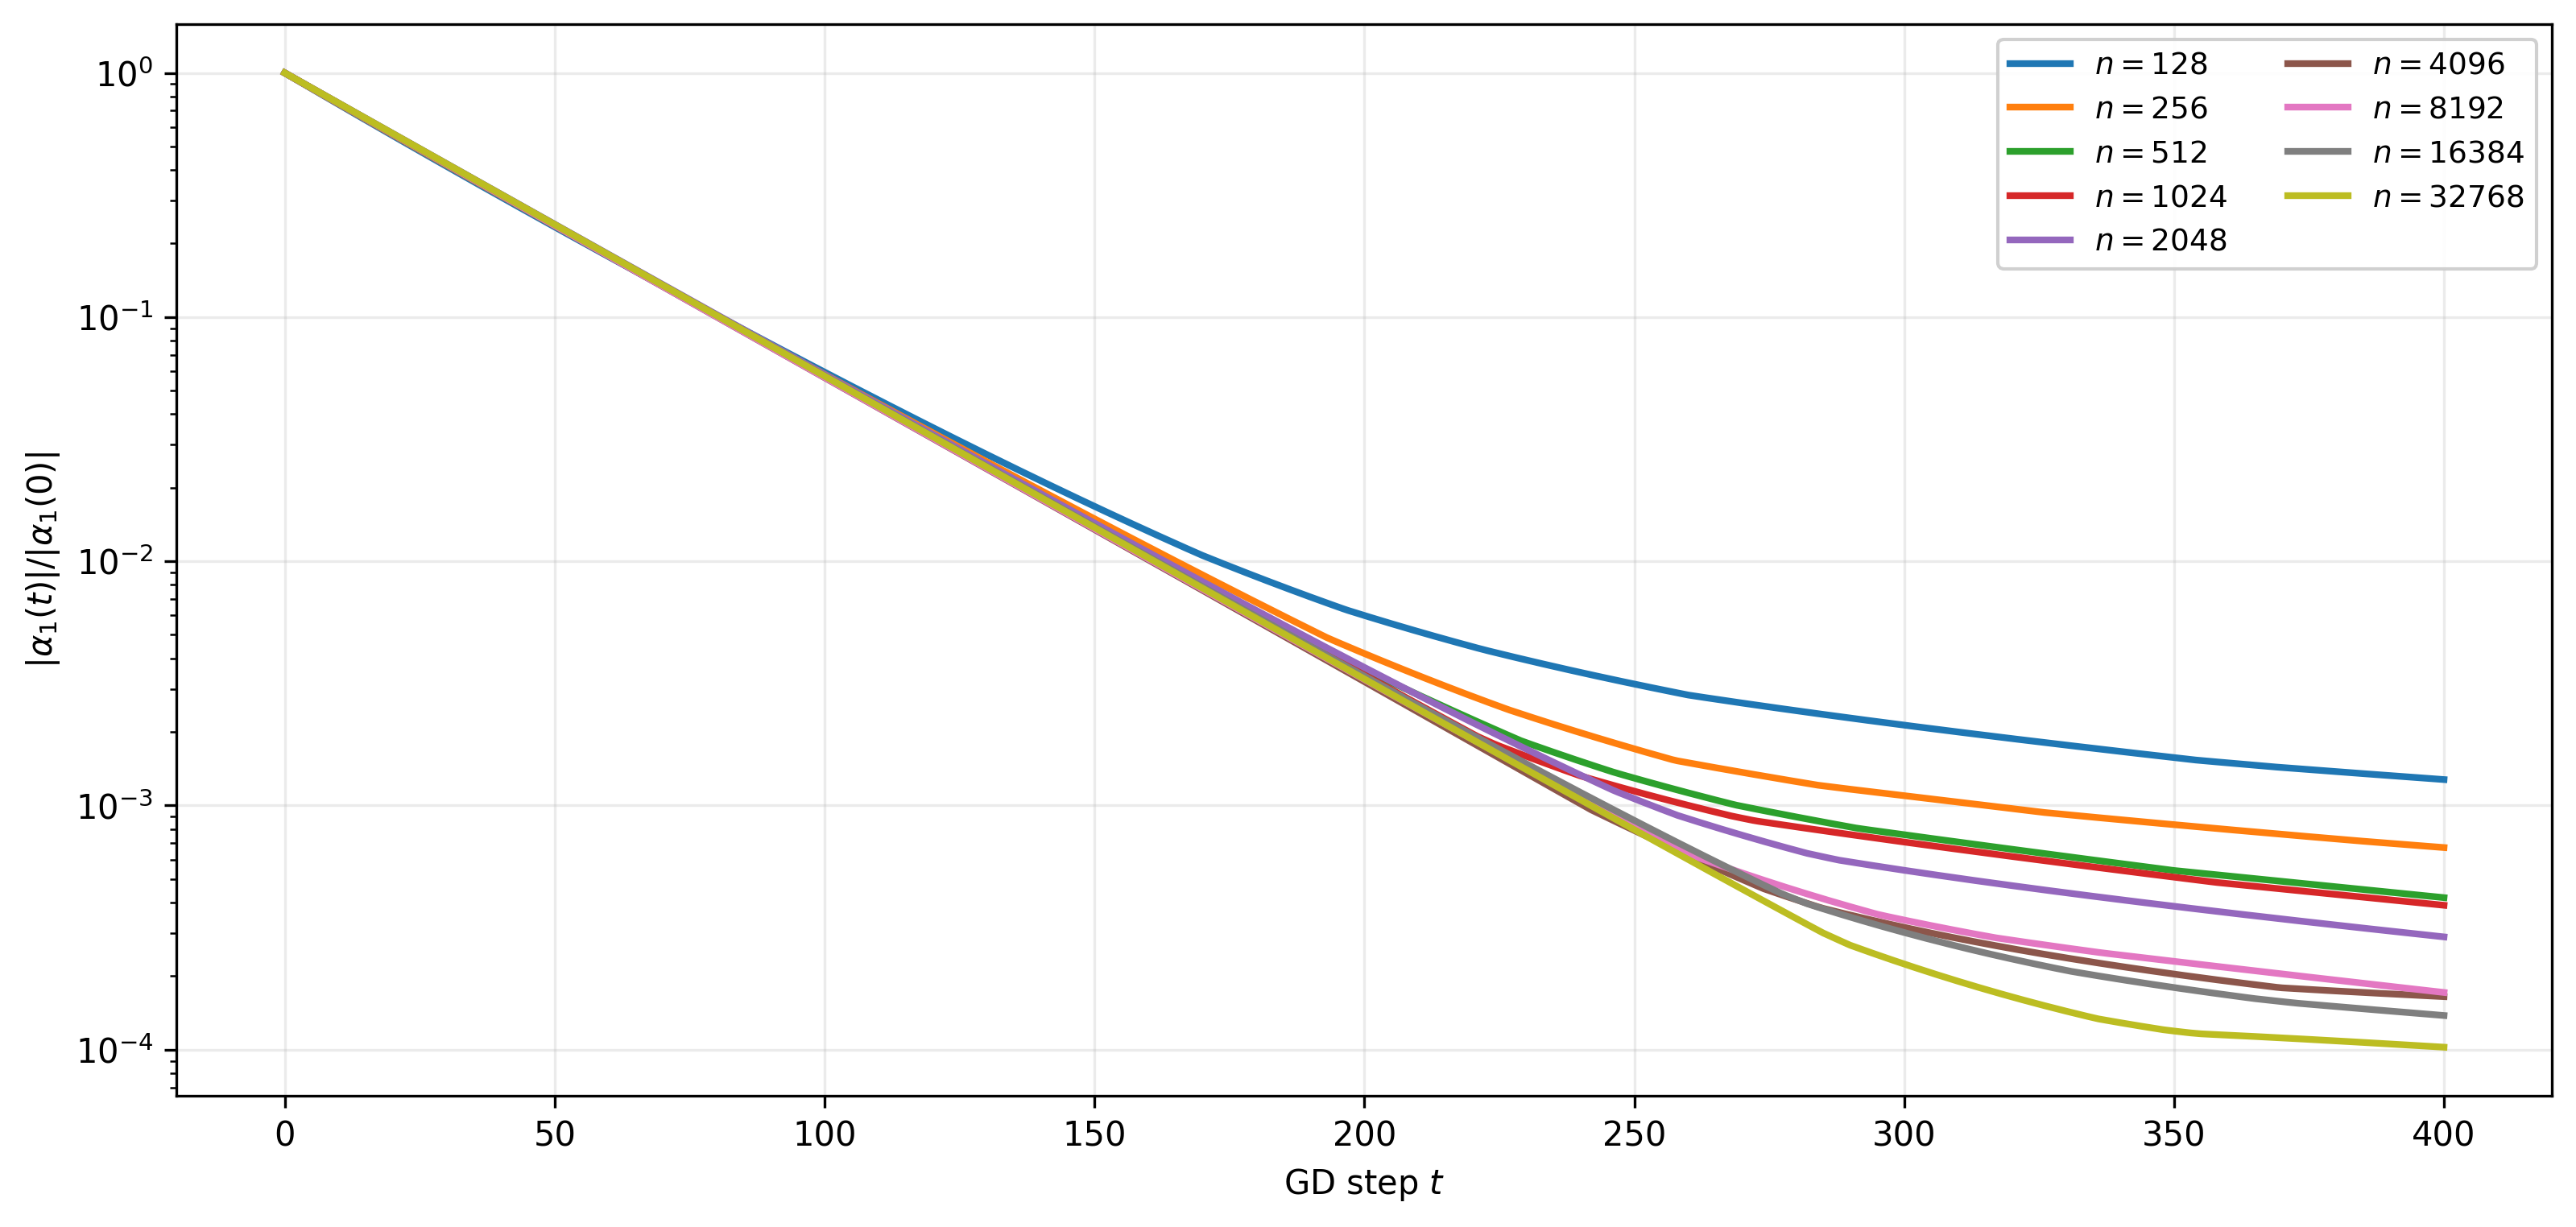
\includegraphics[width=\linewidth]{images/finite_sample_results/story_03_random_high_k1_across_n_first200.png}
    \caption{Normalised residual for mode \(k=1\) over the first 400 gradient steps,
        for sample sizes \(n \in \{128,\ldots,32768\}\).
        Larger \(n\) gives faster effective decay, converging toward the
        continuum rate.}
    \label{fig:app-story03}
\end{figure}

Figure~\ref{fig:app-eig-emp-vs-pred} compares, for a single sample size, the
empirical eigenvalues of the compressed operator \(C=G^{-1}H\) against the
predicted finite-sample eigenvalues \(\lambda_p^{(n)}\).
The predicted values carry the correct Fourier multiplicity: the constant mode
contributes a single eigenvalue, while each frequency \(k\ge 1\) contributes a
degenerate pair, visible as the flat steps in the figure.
The empirical eigenvalues sit on these steps and split only slightly within each
pair, confirming that the sampled operator is close to Fourier-diagonal on the
retained block.
The agreement is tightest for the leading (low-frequency) eigenvalues and
loosens for the smallest eigenvalues, which is where the finite-sample action
error is relatively largest.

\begin{figure}[!htbp]
    \centering
    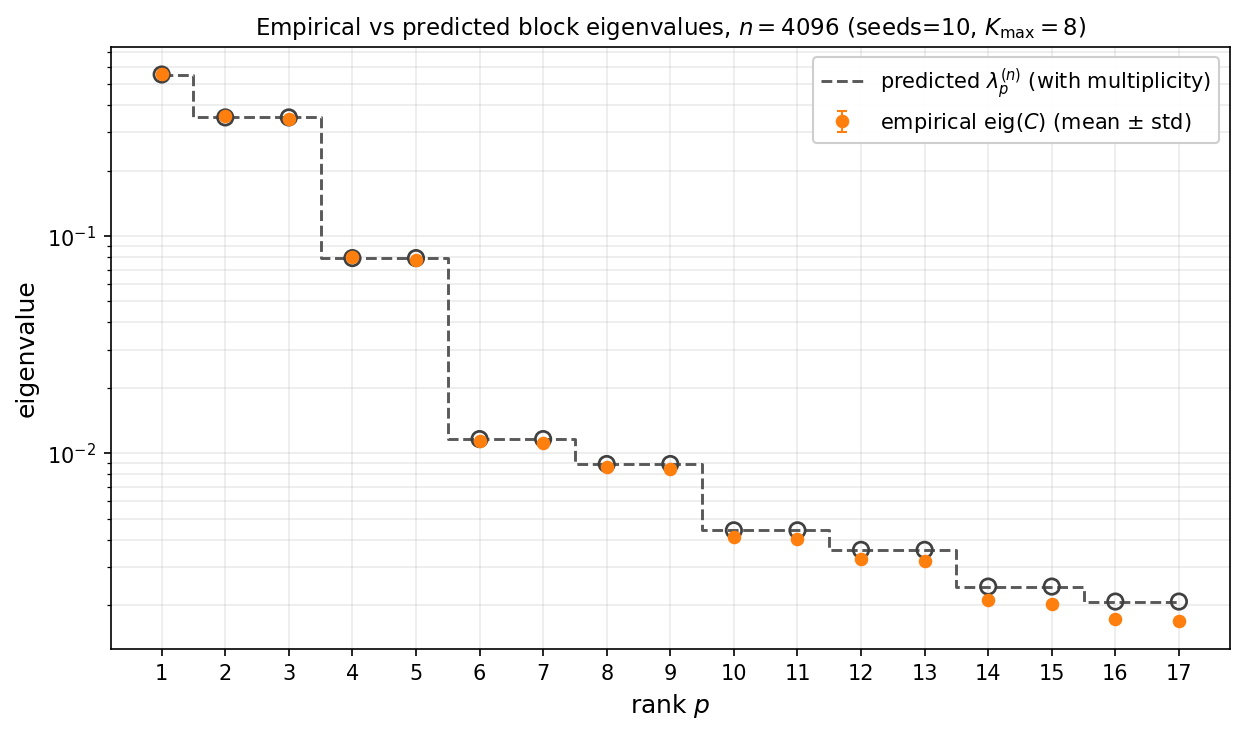
\includegraphics[width=0.82\linewidth]{images/appendix/eigenvalues_empirical_vs_predicted_n4096.png}
    \caption{Empirical versus predicted block eigenvalues at \(n=4096\), on a
        logarithmic scale, averaged over \(10\) seeds.
        The dashed step shows the predicted eigenvalues \(\lambda_p^{(n)}\) with
        their correct multiplicity (single for \(k=0\), degenerate pairs for
        \(k\ge 1\)); markers show the empirical eigenvalues \(\mathrm{eig}(C)\)
        (mean \(\pm\) standard deviation).}
    \label{fig:app-eig-emp-vs-pred}
\end{figure}

Figure~\ref{fig:app-block-spectra} shows the effect of increasing \(n\) on the
block-diagonal structure of the sampled Gram matrix.
The left panel is the baseline spectrum; the centre and right panels show how
the theory- and empirical-preconditioned spectra flatten toward the identity
as \(n\) grows, validating the preconditioner construction.

\begin{figure}[!htbp]
    \centering
    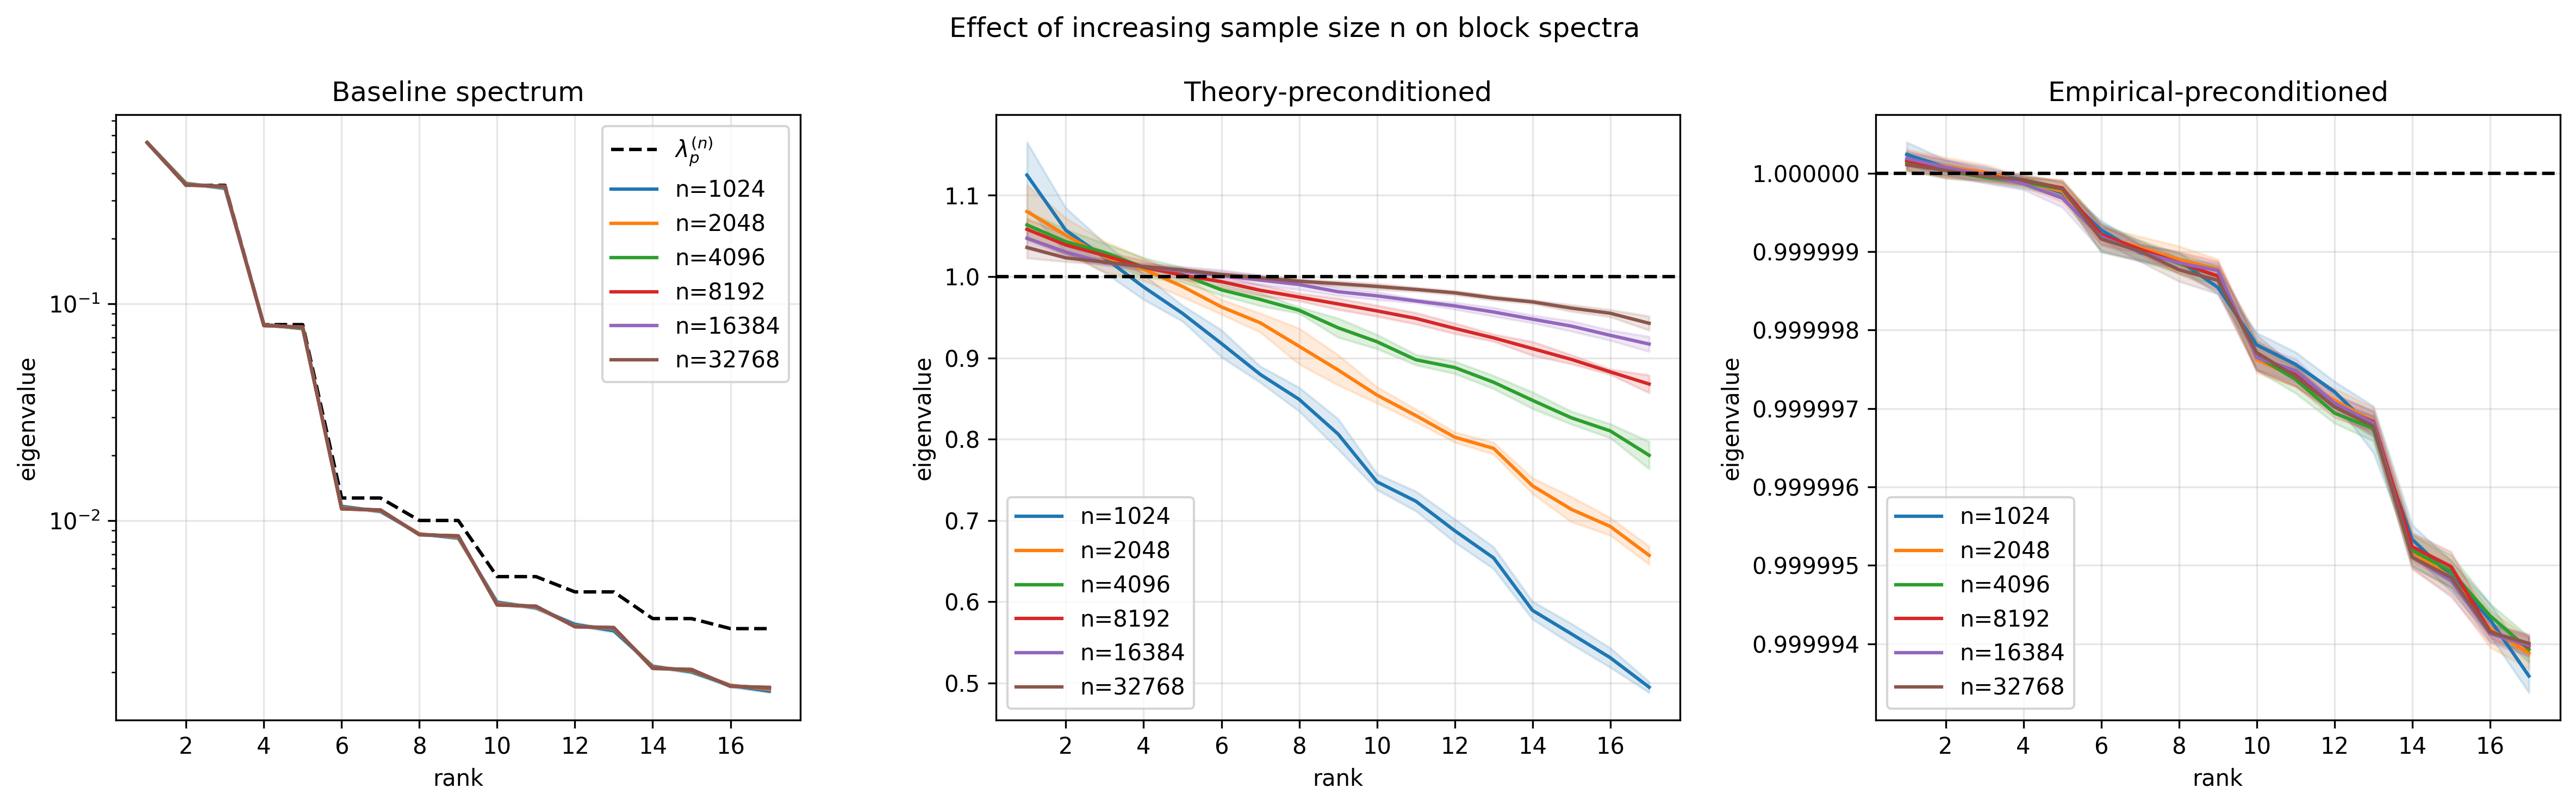
\includegraphics[width=\linewidth]{images/appendix/compressed_block_spectra_all_n.png}
    \caption{Block spectra of the compressed Gram matrix for
        \(n \in \{1024,\ldots,32768\}\).
        Left: baseline (decaying) spectrum.
        Centre: theory-preconditioned spectrum approaching 1.
        Right: empirical-preconditioned spectrum, closely tracking the theory.}
    \label{fig:app-block-spectra}
\end{figure}

Figure~\ref{fig:app-block-spectra-4096} shows the same three spectra for a single
sample size \(n=4096\), annotated with the condition number of each block.
The baseline block is badly conditioned (\(\kappa \approx 1.4\times10^3\)); the
theory preconditioner reduces this to \(\kappa \approx 2.1\), and the empirical
preconditioner flattens the block to \(\kappa \approx 1\).

\begin{figure}[!htbp]
    \centering
    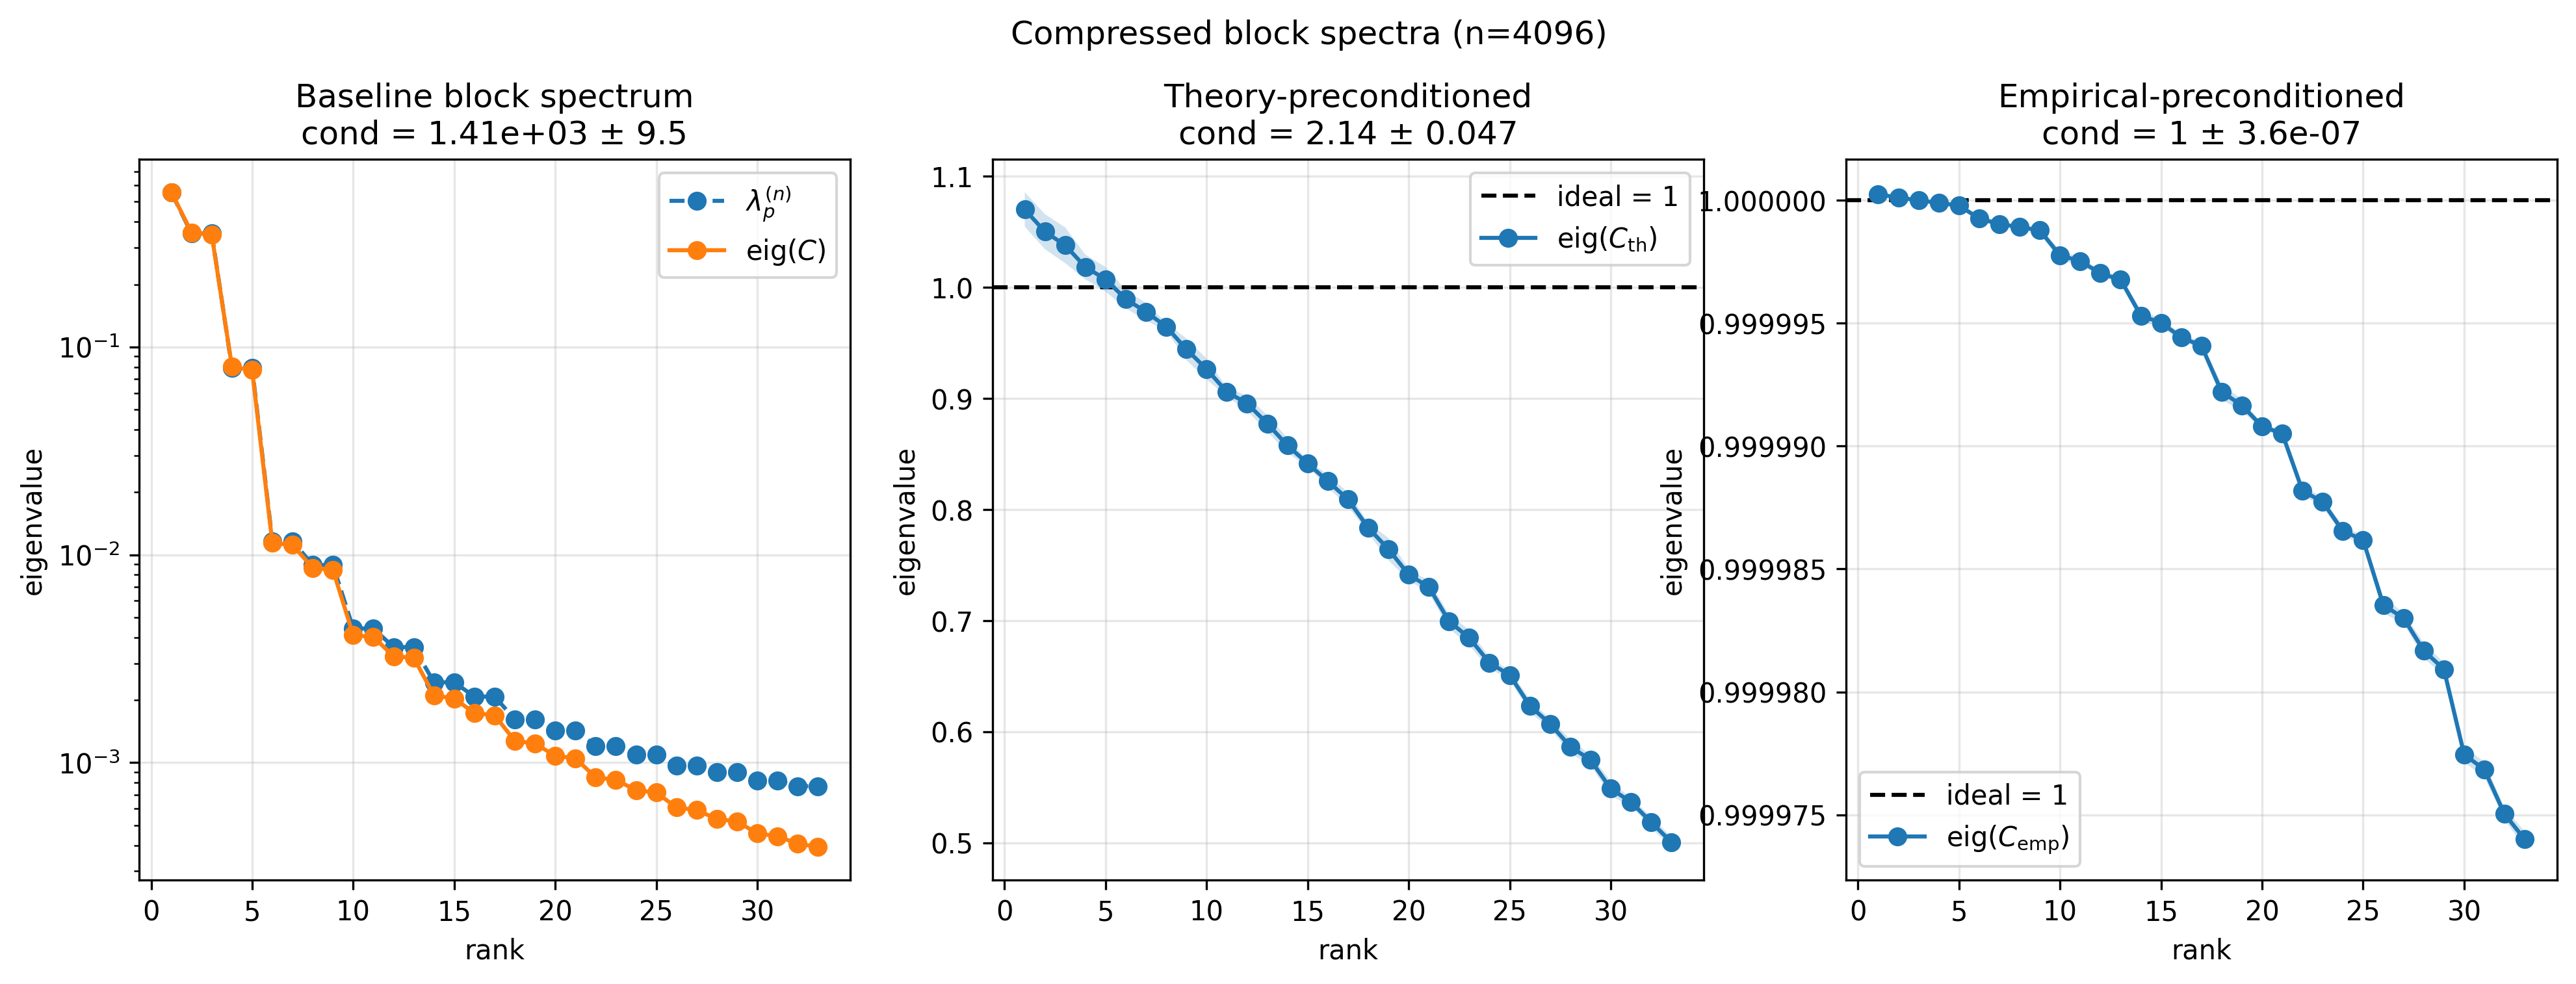
\includegraphics[width=\linewidth]{images/appendix/compressed_block_spectra_4096_all_preconditioned.png}
    \caption{Compressed block spectra at \(n=4096\) with all active modes inside
        the preconditioning block.
        Left: baseline spectrum with a wide spread.
        Centre: theory-preconditioned spectrum, reduced spread but a residual
        slope.
        Right: empirical-preconditioned spectrum, essentially flat at 1.
        Titles report the per-block condition number.}
    \label{fig:app-block-spectra-4096}
\end{figure}

Figures~\ref{fig:app-mode-cos1}--\ref{fig:app-mode-cos7} show the normalised
residual decay for individual Fourier modes under the baseline and both
preconditioned learning rules.
The baseline decay is negligible over 2000 steps for both modes; the
preconditioned rules reduce the residual by several orders of magnitude within
the same budget.

\begin{figure}[!htbp]
    \centering
    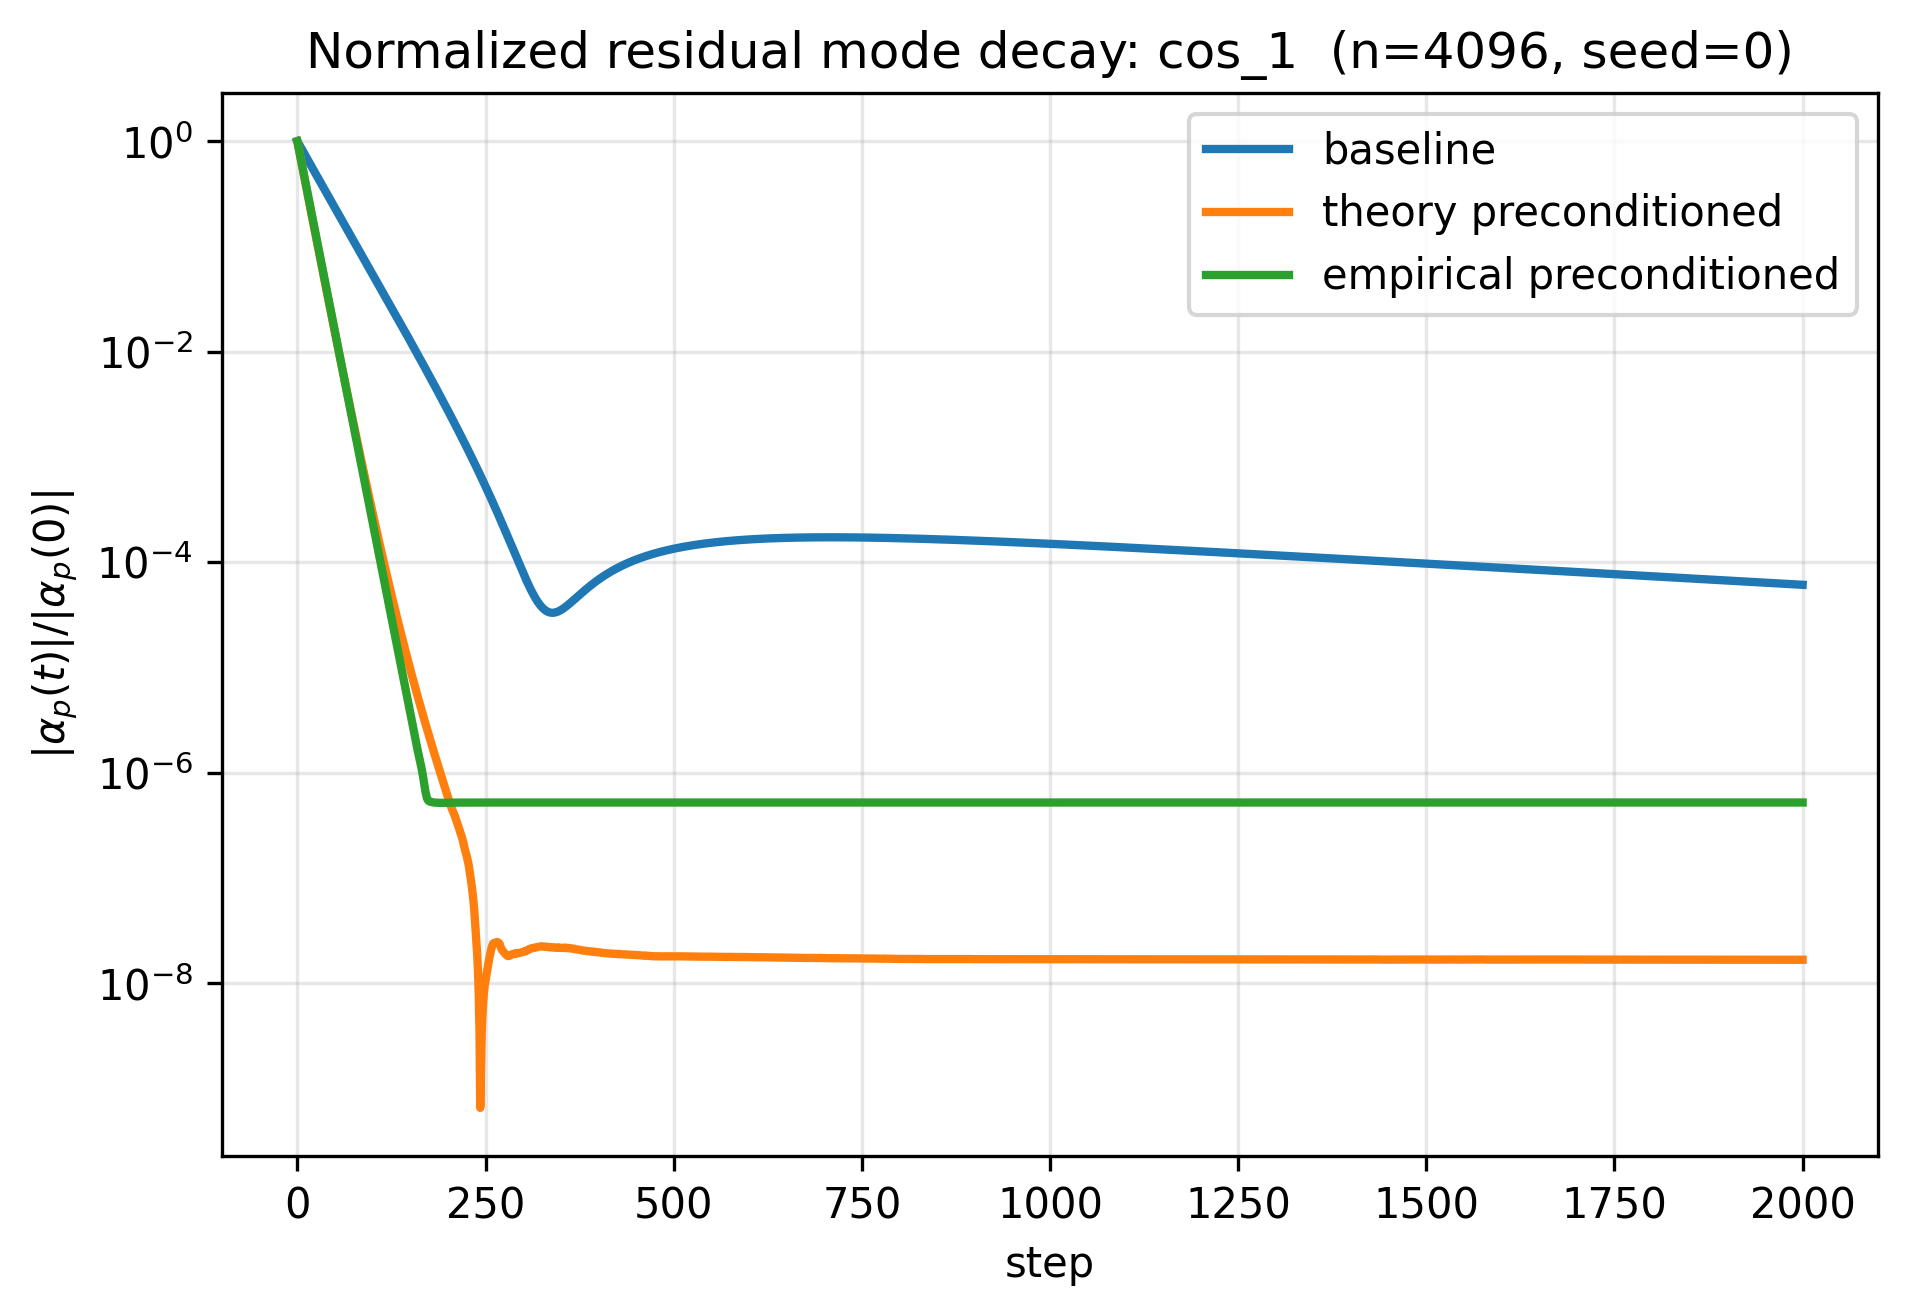
\includegraphics[width=0.72\linewidth]{images/appendix/mode_curve_compare_cos_1_n4096_seed0.png}
    \caption{Per-mode residual decay for \(\cos_1\) (\(n=4096\), seed 0).
        Baseline (blue) is effectively flat; theory-preconditioned (orange)
        and empirical-preconditioned (green) converge rapidly.}
    \label{fig:app-mode-cos1}
\end{figure}

\begin{figure}[!htbp]
    \centering
    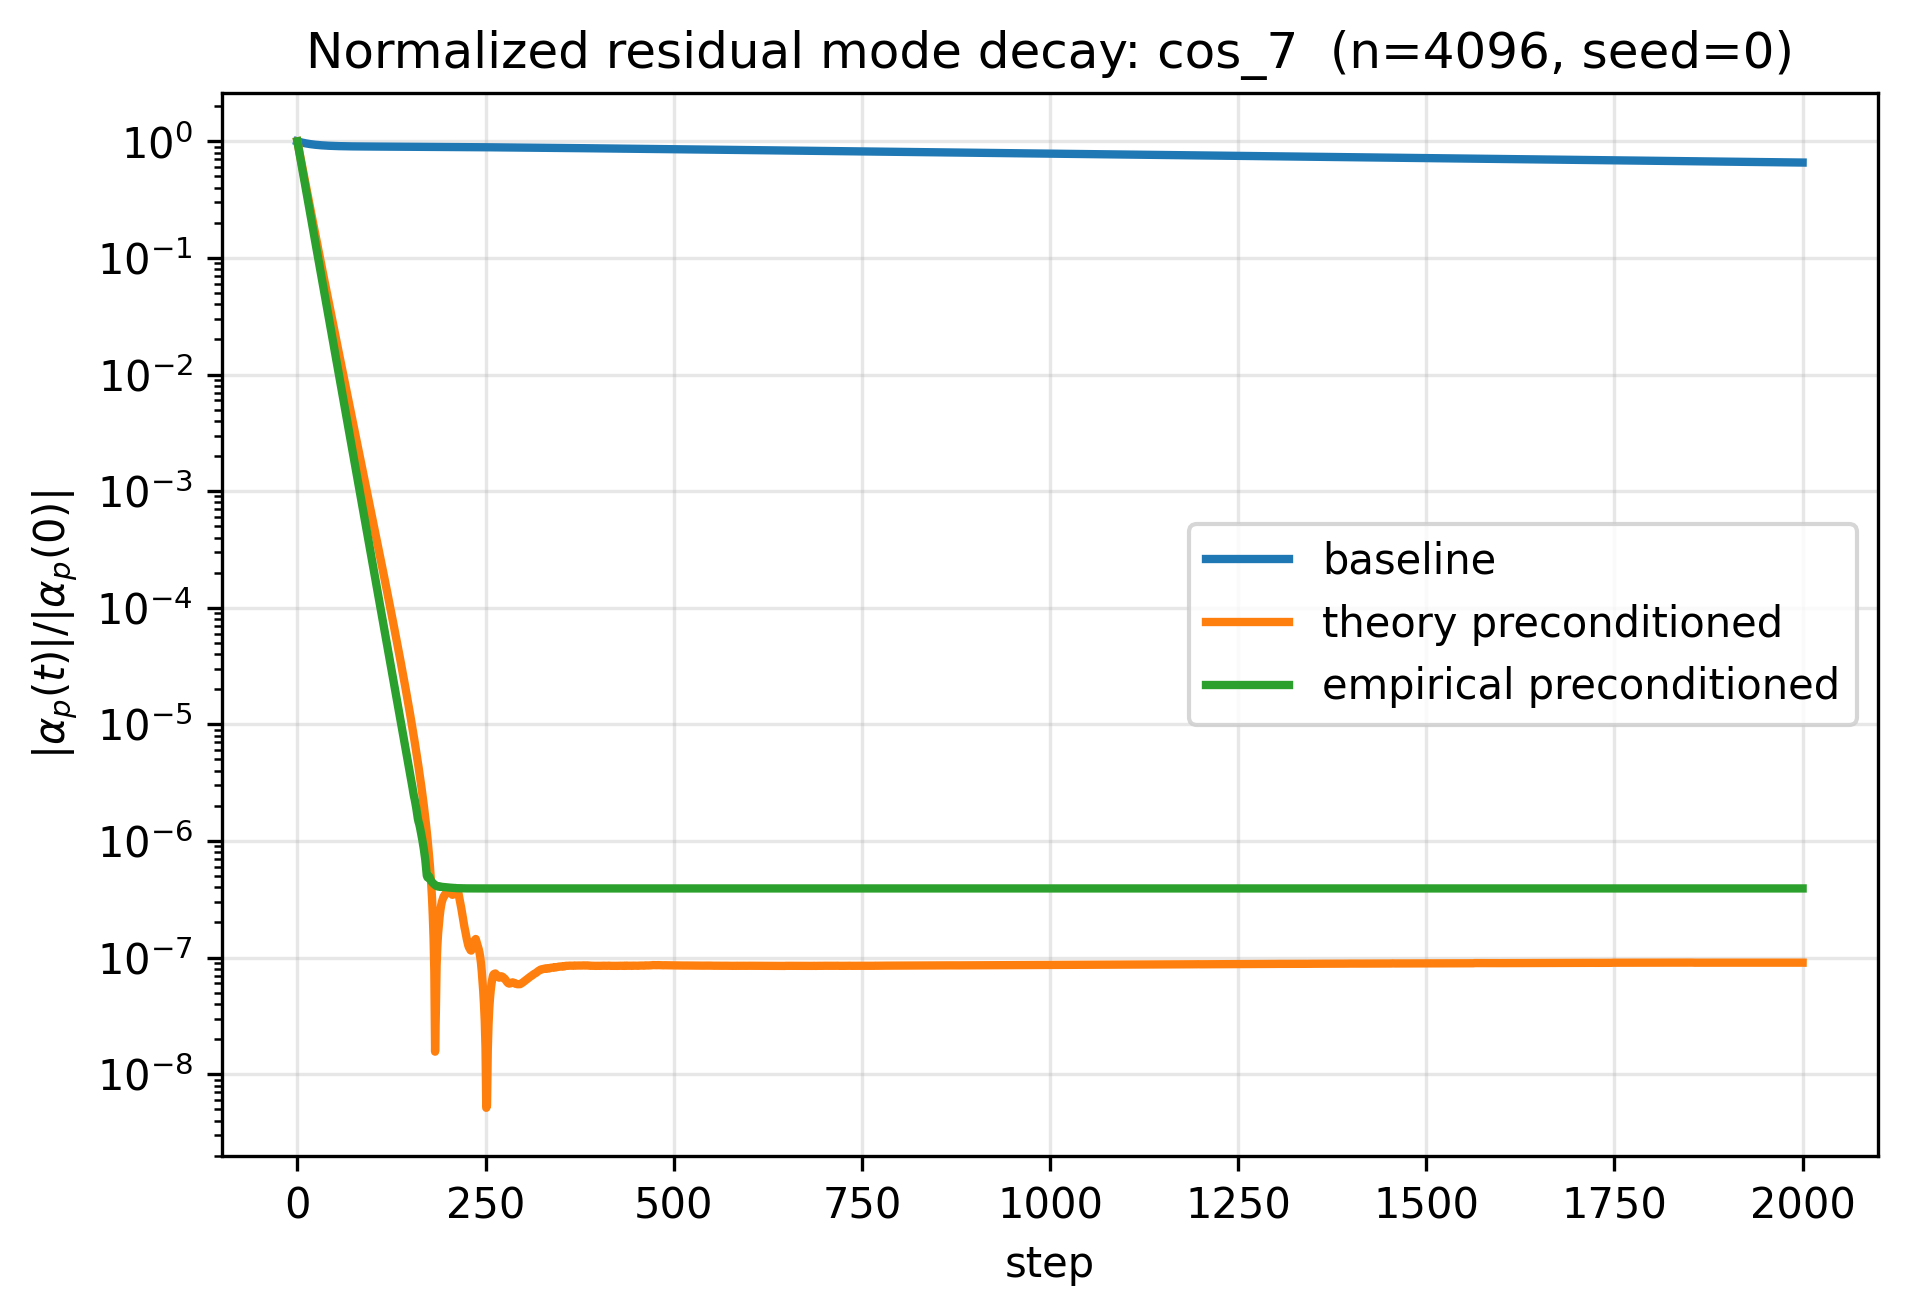
\includegraphics[width=0.72\linewidth]{images/appendix/mode_curve_compare_cos_7_n4096_seed0.png}
    \caption{Per-mode residual decay for \(\cos_7\) (\(n=4096\), seed 0).
        The spectral gap for this higher mode makes the baseline decay
        even slower; preconditioning recovers roughly six orders of magnitude
        of relative residual within 2000 steps.}
    \label{fig:app-mode-cos7}
\end{figure}

% ---------------------------------------------------------------------------
\section{Finite-sample mode decay across sample sizes}
\label{app:add-finite-sample-sweep}

The main text shows the observed-versus-predicted mode decay for a single
sample size \(n=4096\)
(Figures~\ref{fig:results-random-sampling-first200}
and~\ref{fig:results-random-sampling-highfreq}).
Here we repeat the same experiment across the full range of sample sizes
\(n \in \{128,\ldots,32768\}\).
For each \(n\), the left panel shows all retained modes over the first
\(200\) gradient-descent steps, and the right panel isolates the
higher-frequency modes over \(2000\) steps.
Solid curves are the observed normalised residual amplitudes
\(|\alpha_p(t)|/|\alpha_p(0)|\); dashed curves are the diagonal prediction from
the finite-sample corrected eigenvalues \(\lambda_p^{(n)}\).

The trend is consistent with the finite-sample theory.
At small \(n\), the sampled operator is a rough approximation, the prediction
bands are wide, and the observed curves flatten early as the finite-sample
action error becomes comparable to the remaining motion.
As \(n\) grows, the bands tighten and the observed decay tracks the diagonal
prediction over an increasingly long horizon before flattening.

\newcommand{\fssweep}[2]{%
    \begin{figure}[!htbp]
        \centering
        \begin{subfigure}[b]{0.49\linewidth}
            \includegraphics[width=\linewidth]{images/appendix/finite_sample_sweep/story_02_random_n#1_components_first200.png}
            \caption{All modes, first \(200\) steps.}
        \end{subfigure}
        \hfill
        \begin{subfigure}[b]{0.49\linewidth}
            \includegraphics[width=\linewidth]{images/appendix/finite_sample_sweep/story_02_random_n#1_components_all_steps_high_freq_only.png}
            \caption{Higher-frequency modes, \(2000\) steps.}
        \end{subfigure}
        \caption{Random sampling with \(n=#1\): observed (solid) versus
            finite-sample eigenvalue prediction (dashed). #2}
        \label{fig:app-fs-sweep-n#1}
    \end{figure}%
}

\fssweep{128}{The prediction bands are wide and the observed curves flatten
    early.}
\fssweep{256}{}
\fssweep{512}{}
\fssweep{1024}{The observed decay already tracks the prediction over most of the
    early window.}
\fssweep{2048}{}
\fssweep{8192}{}
\fssweep{16384}{}
\fssweep{32768}{At the largest sample size the bands are tight and the agreement
    with the diagonal prediction is closest.}

% ---------------------------------------------------------------------------
\section{Frozen-kernel Fourier eigenspace alignment}
\label{app:add-eigenspace-alignment}

The frozen-kernel analysis assumes that the initial finite-width operator already
reproduces the Fourier spectral structure of the infinite-width theory.
This section examines how well that assumption holds frequency by frequency.
For each \(k\ge 1\), the ideal eigenspace is the two-dimensional Fourier plane
\(\mathcal F_k = \operatorname{span}\{\phi_{k,c},\phi_{k,s}\}\), so the comparison
must be made at the level of subspaces rather than individual eigenvectors:
even a perfectly recovered frequency block has an arbitrary orthonormal basis
inside \(\mathcal F_k\).
We therefore use two basis-free diagnostics, the principal angles between the
empirical eigenspace and \(\mathcal F_k\), and the projector error
\(\|\widehat P_k - P_k\|_F\).

An important caveat is that eigenvalue agreement alone does not certify
eigenspace recovery.
Figure~\ref{fig:app-eigval-vs-freq} shows that the eigenvalue alignment error and
the empirical pair-splitting both decrease quickly with width, yet these
quantities can be small at high frequencies while the corresponding eigenspaces
are still poorly aligned.

\begin{figure}[!htbp]
    \centering
    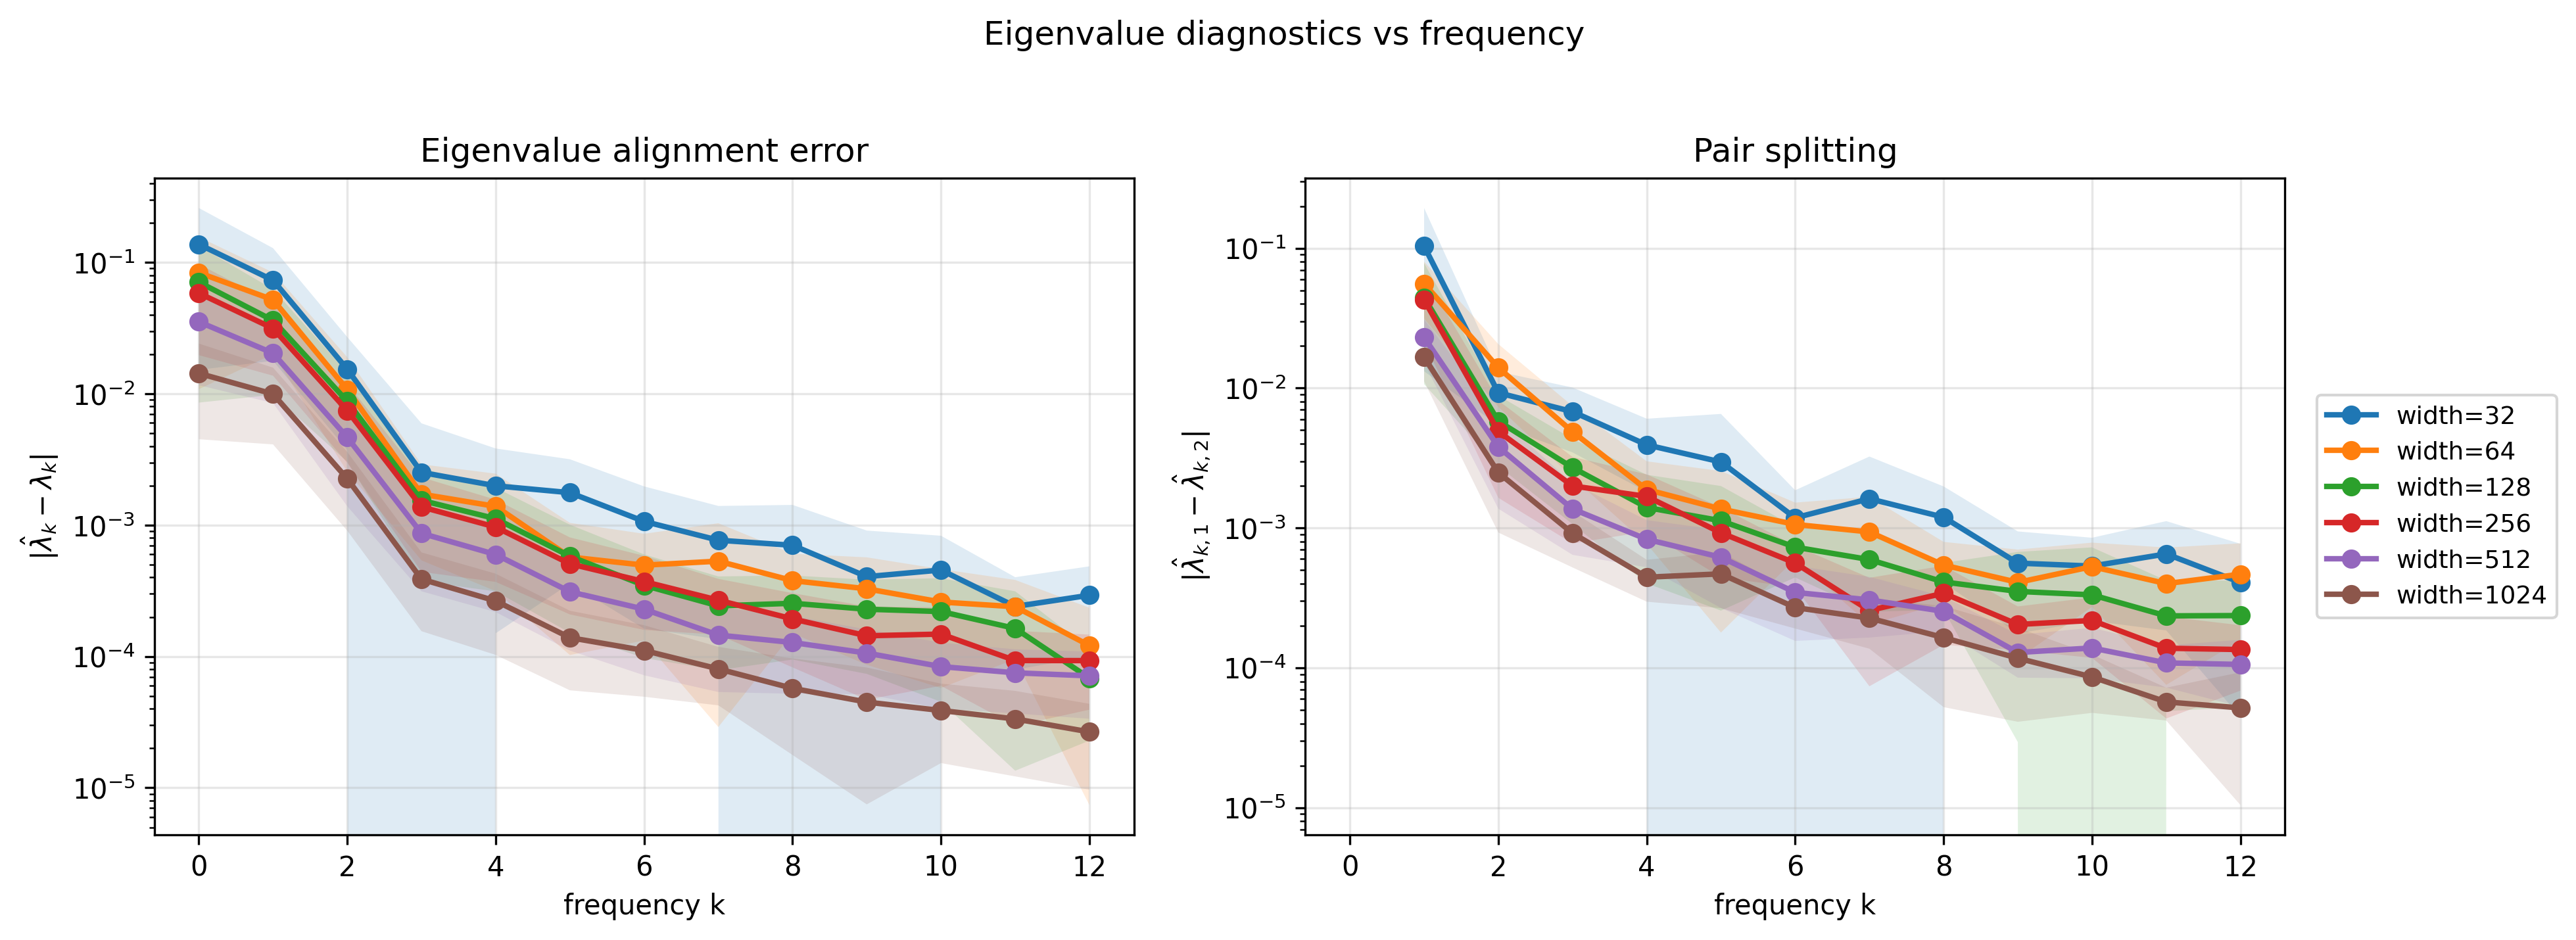
\includegraphics[width=0.92\linewidth]{images/appendix/eigenspace_alignment/eigenvalue_error_vs_frequency.png}
    \caption{Eigenvalue diagnostics for the frozen empirical kernel versus
        frequency, across widths.
        Left: absolute eigenvalue alignment error \(|\widehat\lambda_k-\lambda_k|\).
        Right: empirical splitting of the degenerate \(k\)-pair
        \(|\widehat\lambda_{k,1}-\widehat\lambda_{k,2}|\).
        Both shrink with width, but small eigenvalue error alone does not imply
        good eigenspace recovery.}
    \label{fig:app-eigval-vs-freq}
\end{figure}

The eigenspace diagnostics show a clear frequency hierarchy.
Figure~\ref{fig:app-eigvec-shapes} compares the mean empirical eigenvectors with
the Fourier targets at width \(256\): the low frequencies are tracked closely,
while phase and amplitude distortions grow with \(k\).
Figure~\ref{fig:app-fourier-plane} shows the same effect in the raw Fourier
plane, where the low-frequency clouds lie near the unit circle and higher
frequencies drift inward.
Figure~\ref{fig:app-projerr-freq} summarises this as a projector error that grows
rapidly with \(k\): only the lowest modes are recovered accurately at the widths
considered here.

\begin{figure}[!htbp]
    \centering
    \includegraphics[width=0.92\linewidth]{images/appendix/eigenspace_alignment/eigenvector_shape_grid_7x6_w256.png}
    \caption{Mean empirical eigenvector components (orange) versus the Fourier
        targets (black) at width \(256\), with one-standard-deviation bands over
        seeds. Low frequencies are tracked closely; distortion and variability
        grow with frequency.}
    \label{fig:app-eigvec-shapes}
\end{figure}

\begin{figure}[!htbp]
    \centering
    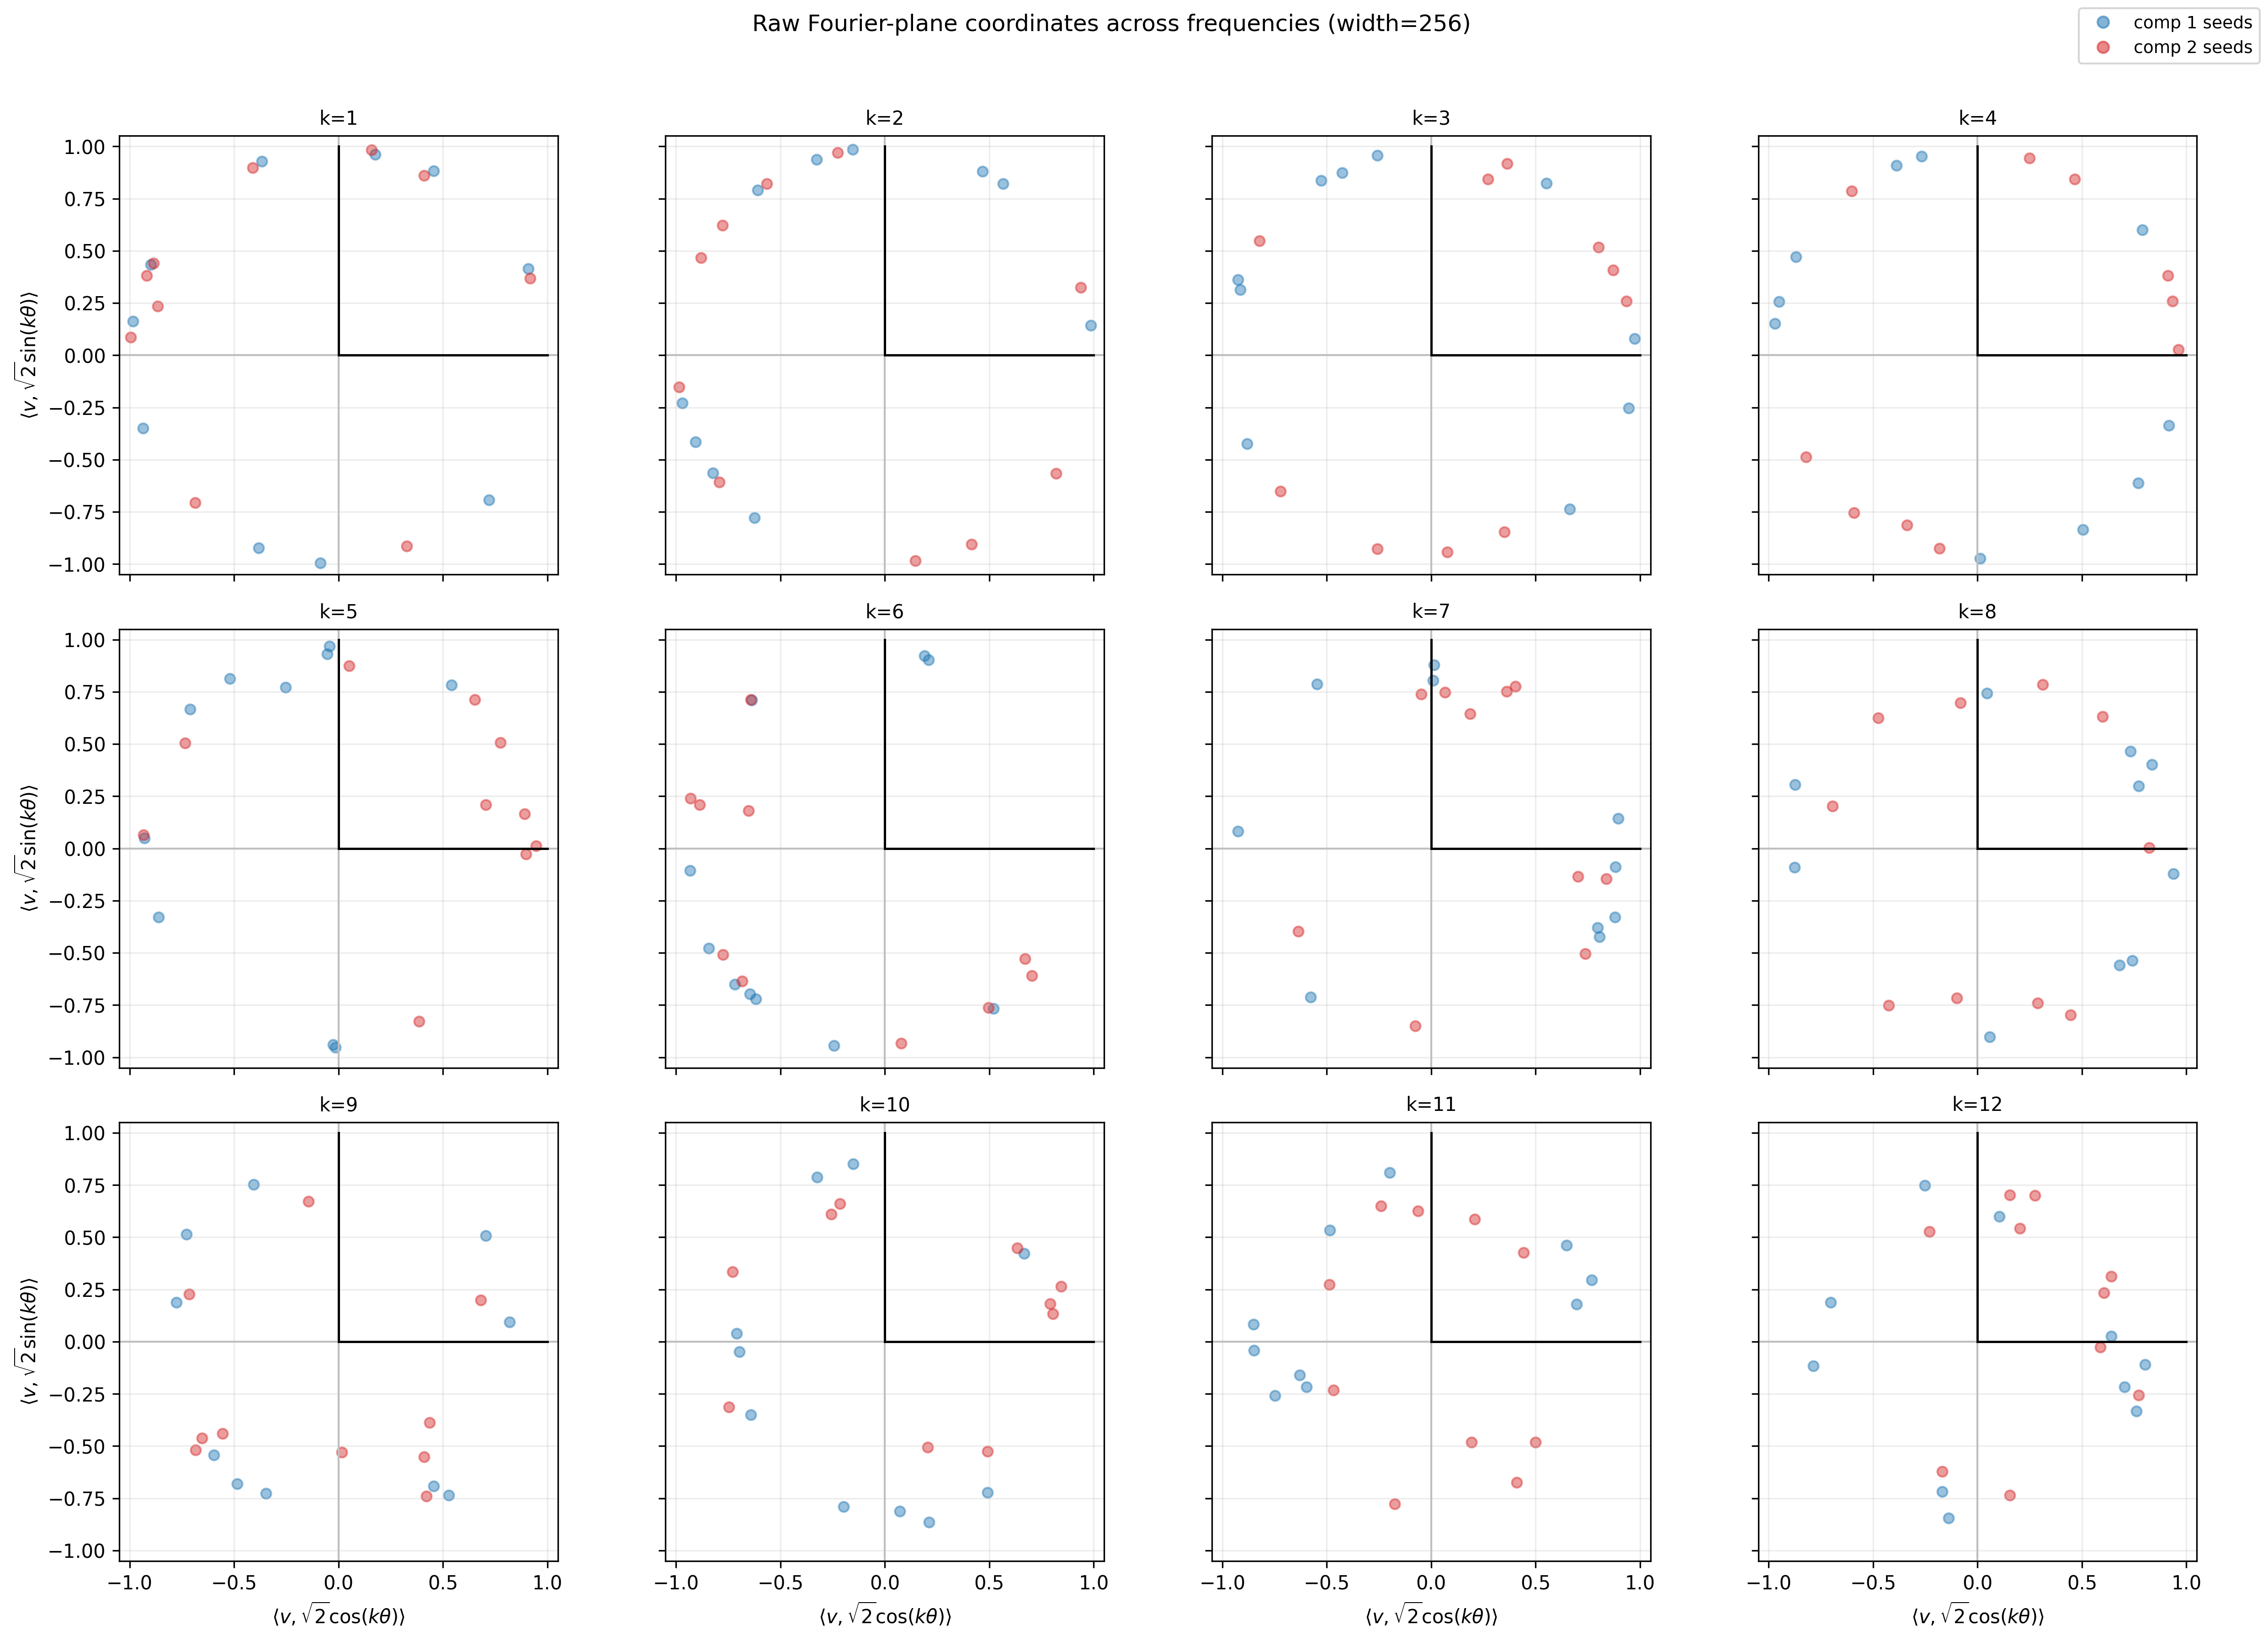
\includegraphics[width=0.92\linewidth]{images/appendix/eigenspace_alignment/eigenvector_fourier_plane_raw_multi_freq_w256.png}
    \caption{Raw Fourier-plane coordinates of the empirical eigenvectors across
        frequencies at width \(256\). Points near the unit circle lie mostly
        inside \(\mathcal F_k\); inward drift indicates leakage outside the
        Fourier plane.}
    \label{fig:app-fourier-plane}
\end{figure}

\begin{figure}[!htbp]
    \centering
    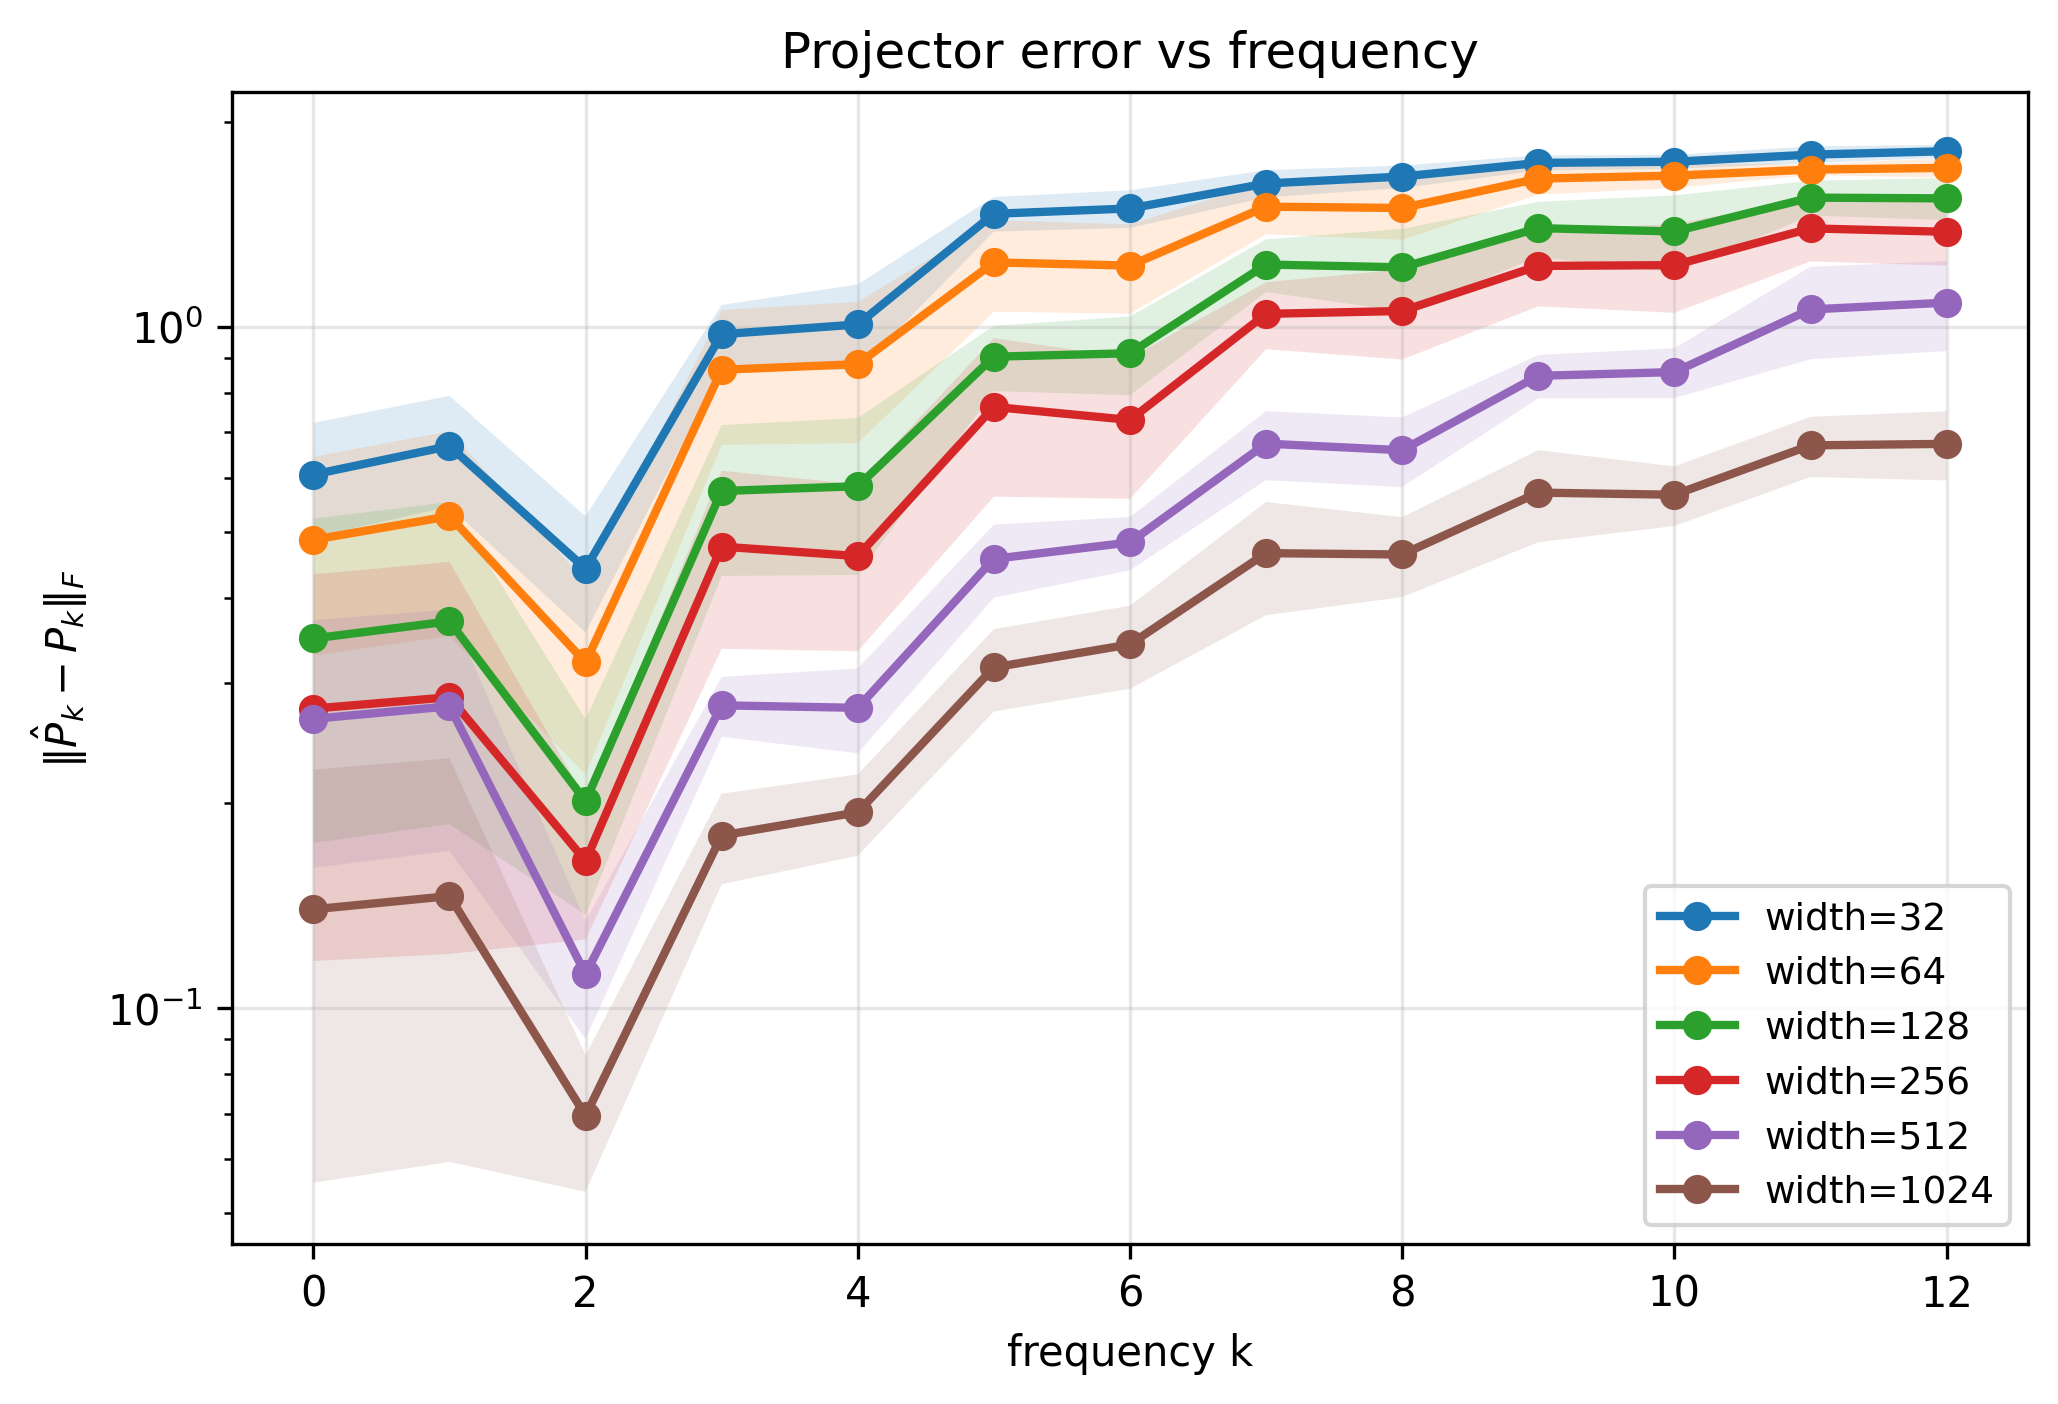
\includegraphics[width=0.92\linewidth]{images/appendix/eigenspace_alignment/projector_error_vs_frequency.png}
    \caption{Projector error \(\|\widehat P_k-P_k\|_F\) versus frequency for
        several widths. The error grows rapidly with \(k\): subspace recovery
        deteriorates at higher frequencies even when the lowest modes are well
        aligned.}
    \label{fig:app-projerr-freq}
\end{figure}

When the kernel is allowed to evolve, the empirical eigenspaces move \emph{away}
from the Fourier planes rather than toward them, even as the network optimises
better than the frozen baseline.
Figure~\ref{fig:app-principal-angles-training} shows the principal angles
increasing during training at width \(256\), with the largest drift at \(k=5\)
and \(k=6\); Figure~\ref{fig:app-raw-grid-evolving} shows the same drift in the
raw Fourier plane.
This is consistent with the interpretation that feature learning helps through
spectral reweighting rather than by preserving the Fourier geometry.

\begin{figure}[!htbp]
    \centering
    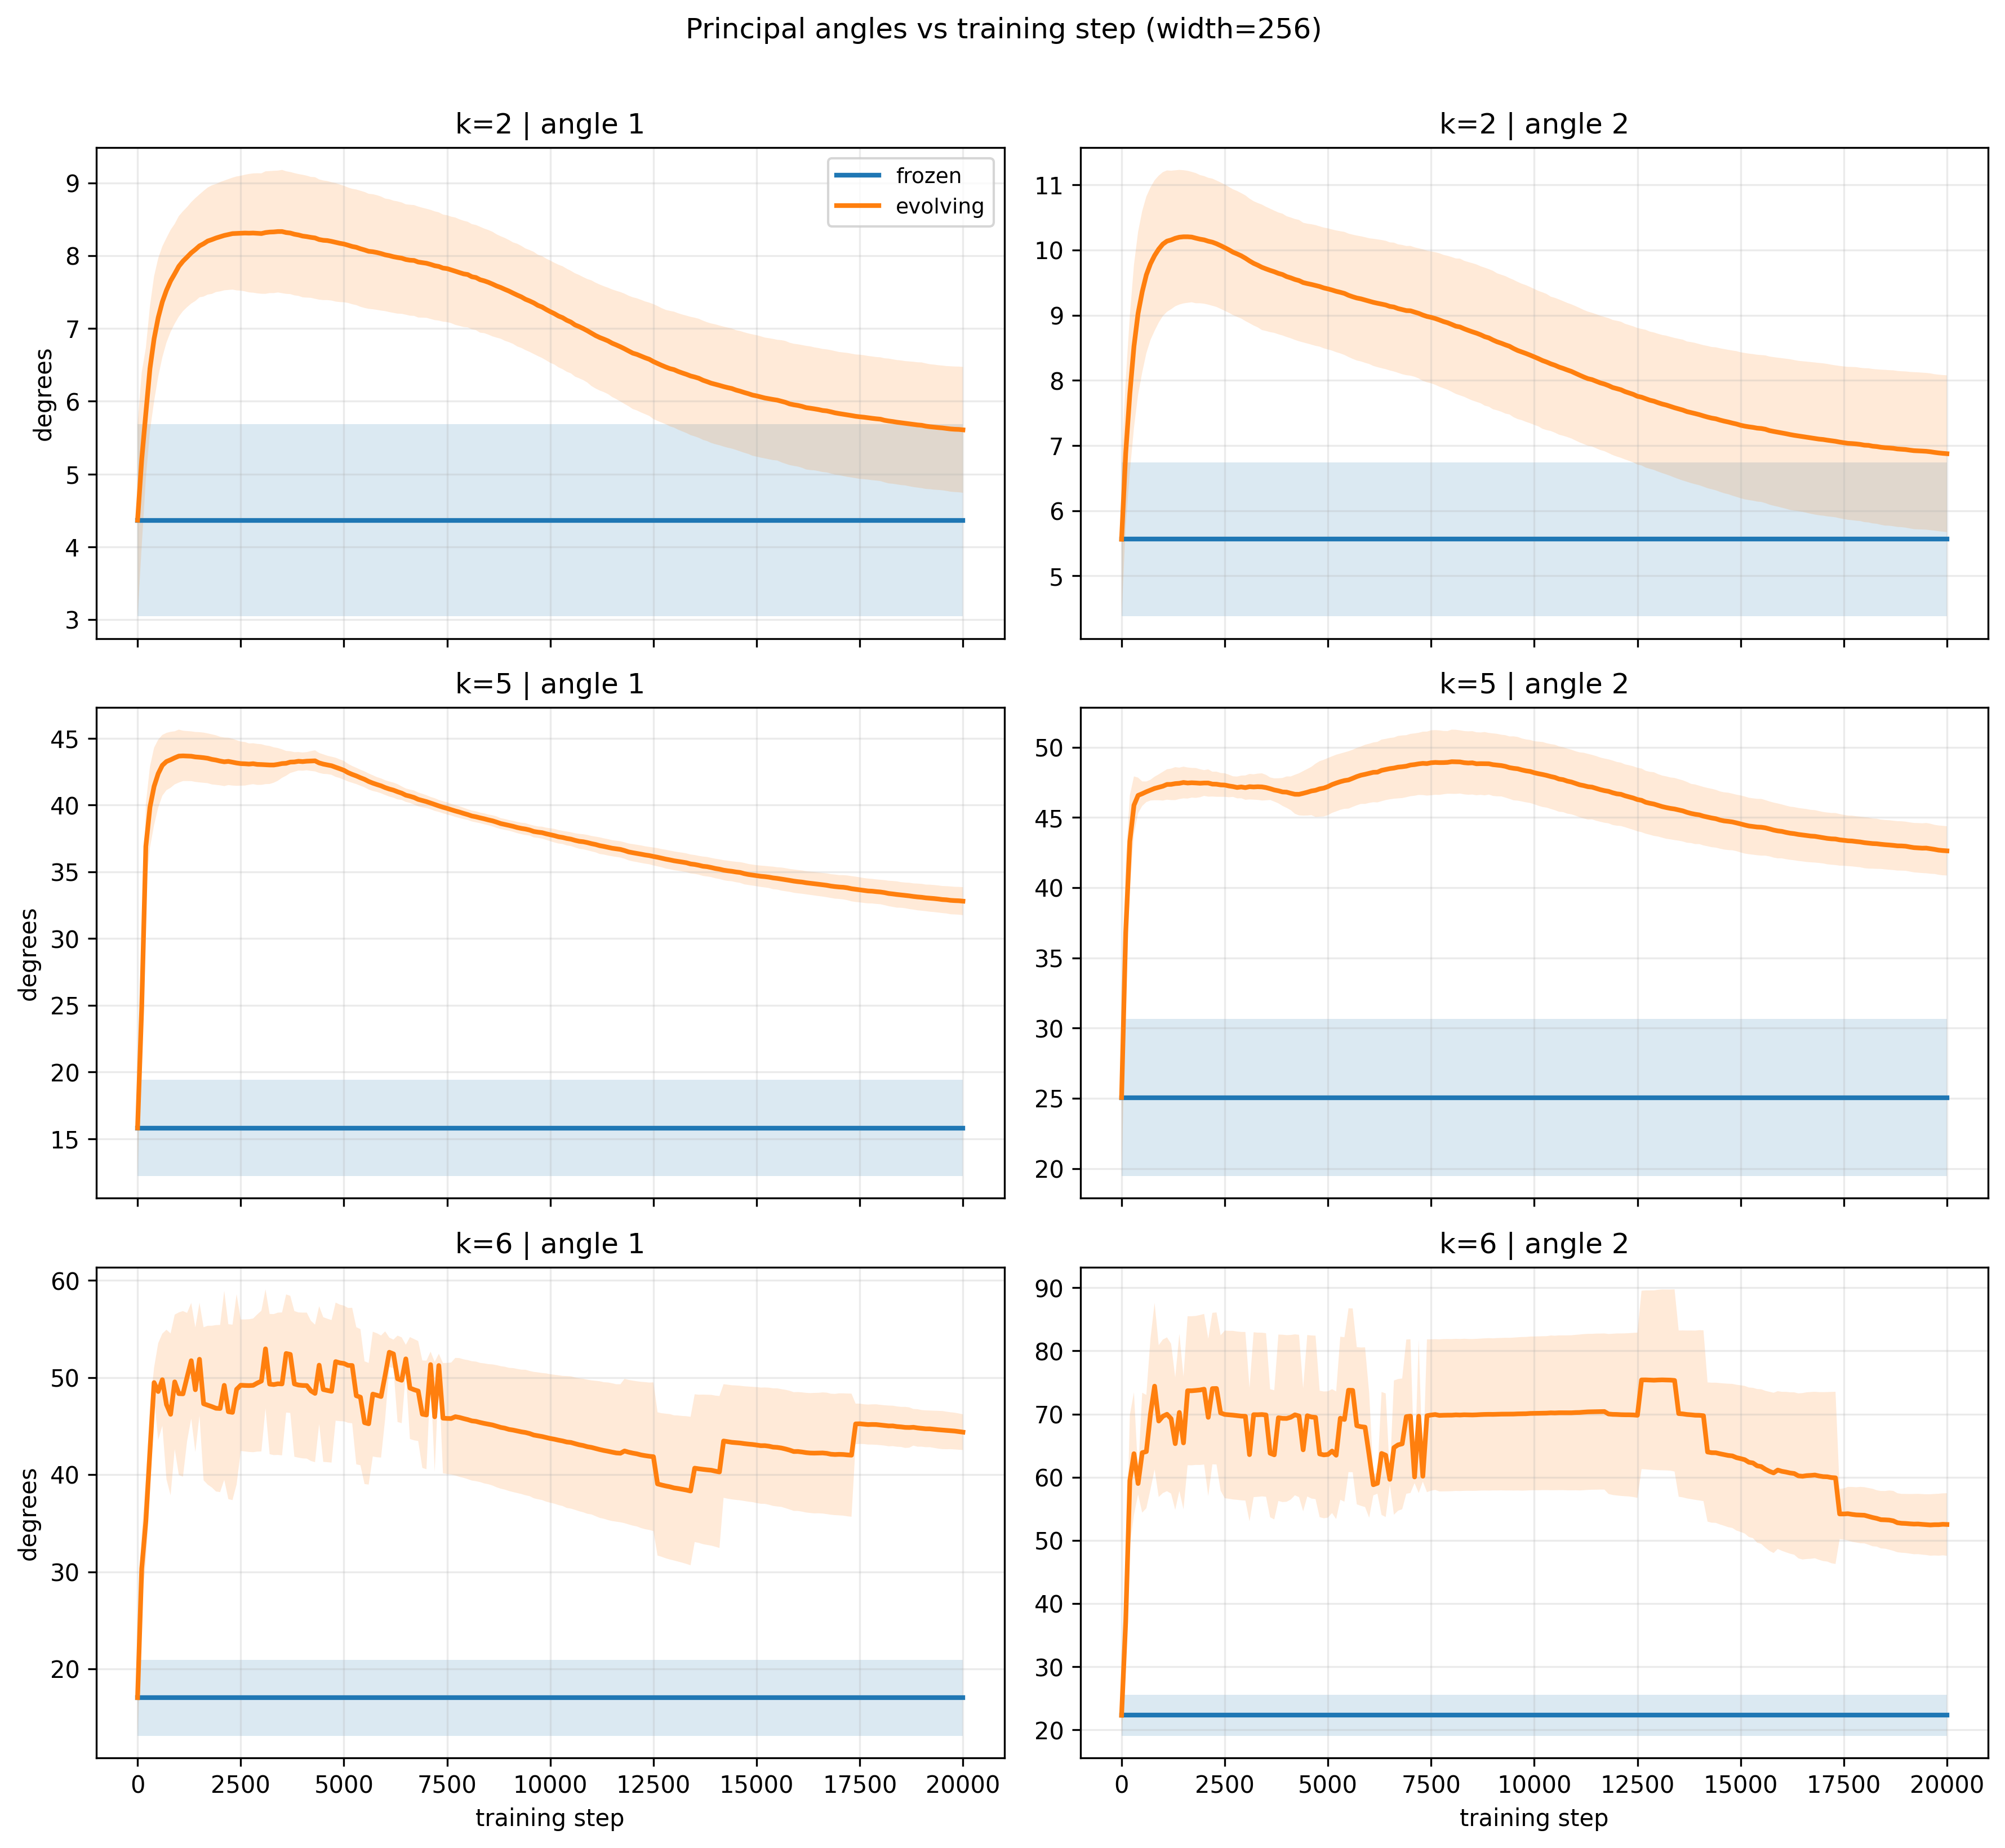
\includegraphics[width=\linewidth]{images/appendix/eigenspace_alignment/principal_angles_over_training_w256.png}
    \caption{Principal angles between the empirical eigenspaces and the Fourier
        planes during training at width \(256\). The frozen branch is constant by
        construction; the evolving branch departs immediately, with the largest
        drift at \(k=5\) and \(k=6\).}
    \label{fig:app-principal-angles-training}
\end{figure}

\begin{figure}[!htbp]
    \centering
    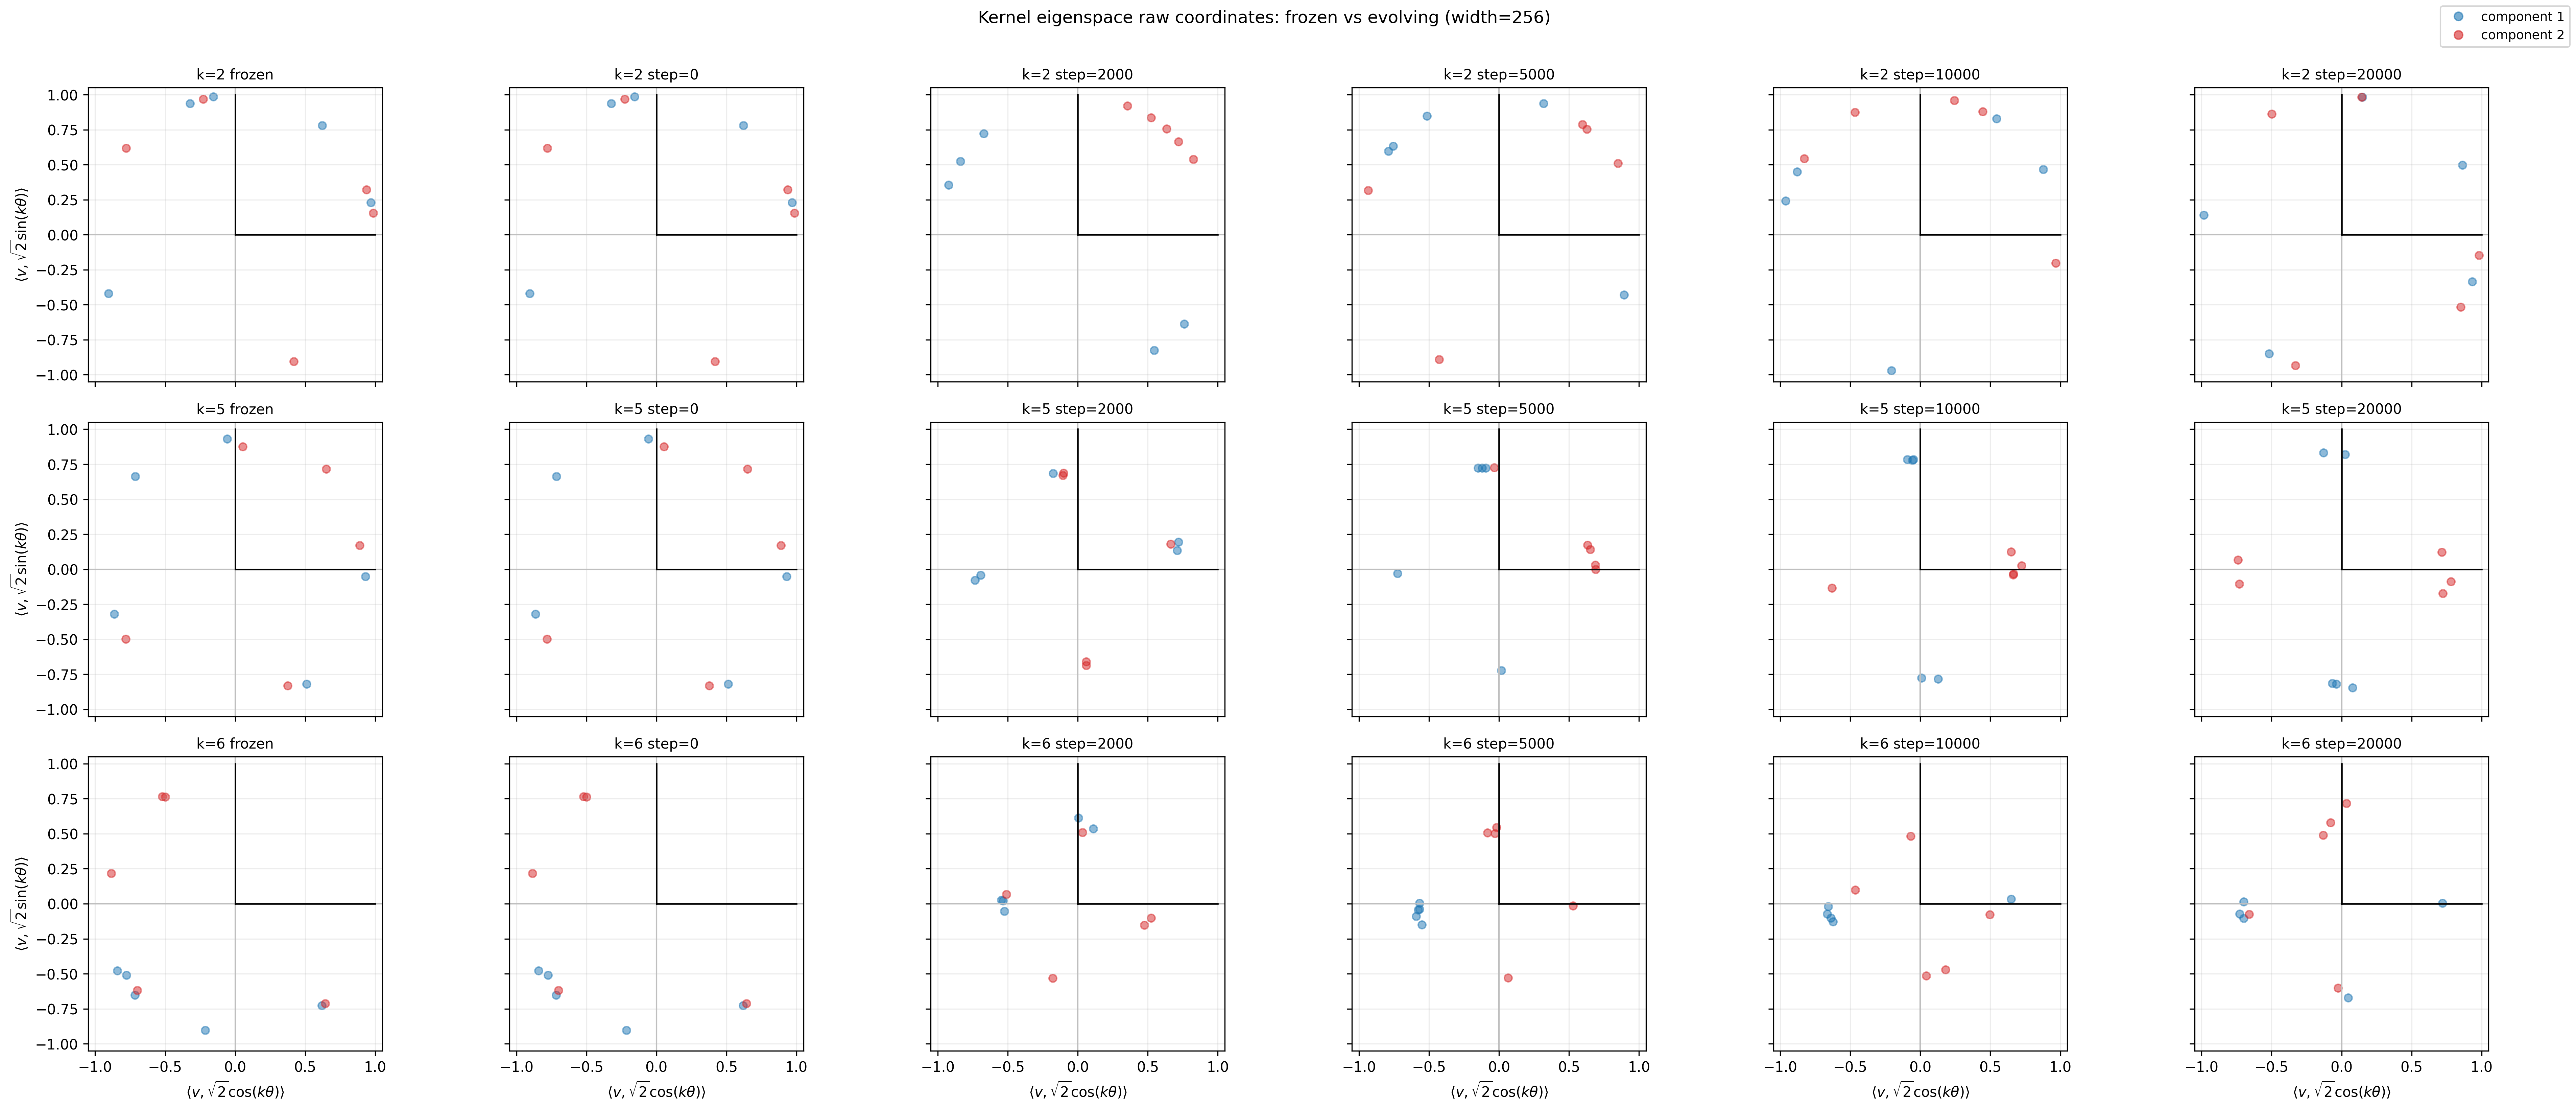
\includegraphics[width=\linewidth]{images/appendix/eigenspace_alignment/raw_kernel_eigenspace_grid_frozen_vs_evolving_w256.png}
    \caption{Raw Fourier-plane coordinates of the empirical eigenspaces for
        \(k=2,5,6\), comparing the frozen baseline with the evolving branch at
        several training steps (width \(256\)). The frozen and step-\(0\) columns
        coincide; the \(k=5\) and \(k=6\) eigenspaces reorganise away from the
        initial Fourier pattern.}
    \label{fig:app-raw-grid-evolving}
\end{figure}

% ---------------------------------------------------------------------------
\section{Finite-width frozen: projector stability}
\label{app:add-projector-stability}

The frozen-NTK analysis relies on the eigenspaces of \(C_0\) remaining close
to those of \(C_t\) throughout training.
Figure~\ref{fig:app-proj-err} confirms this directly: the absolute projection
error \(\|\hat P_k(t) - \hat P_k(0)\|_F\) stays close to zero for the frozen
network at both widths, while it grows for the evolving network, especially at
the smallest width.

\begin{figure}[!htbp]
    \centering
    \begin{subfigure}[b]{0.49\linewidth}
        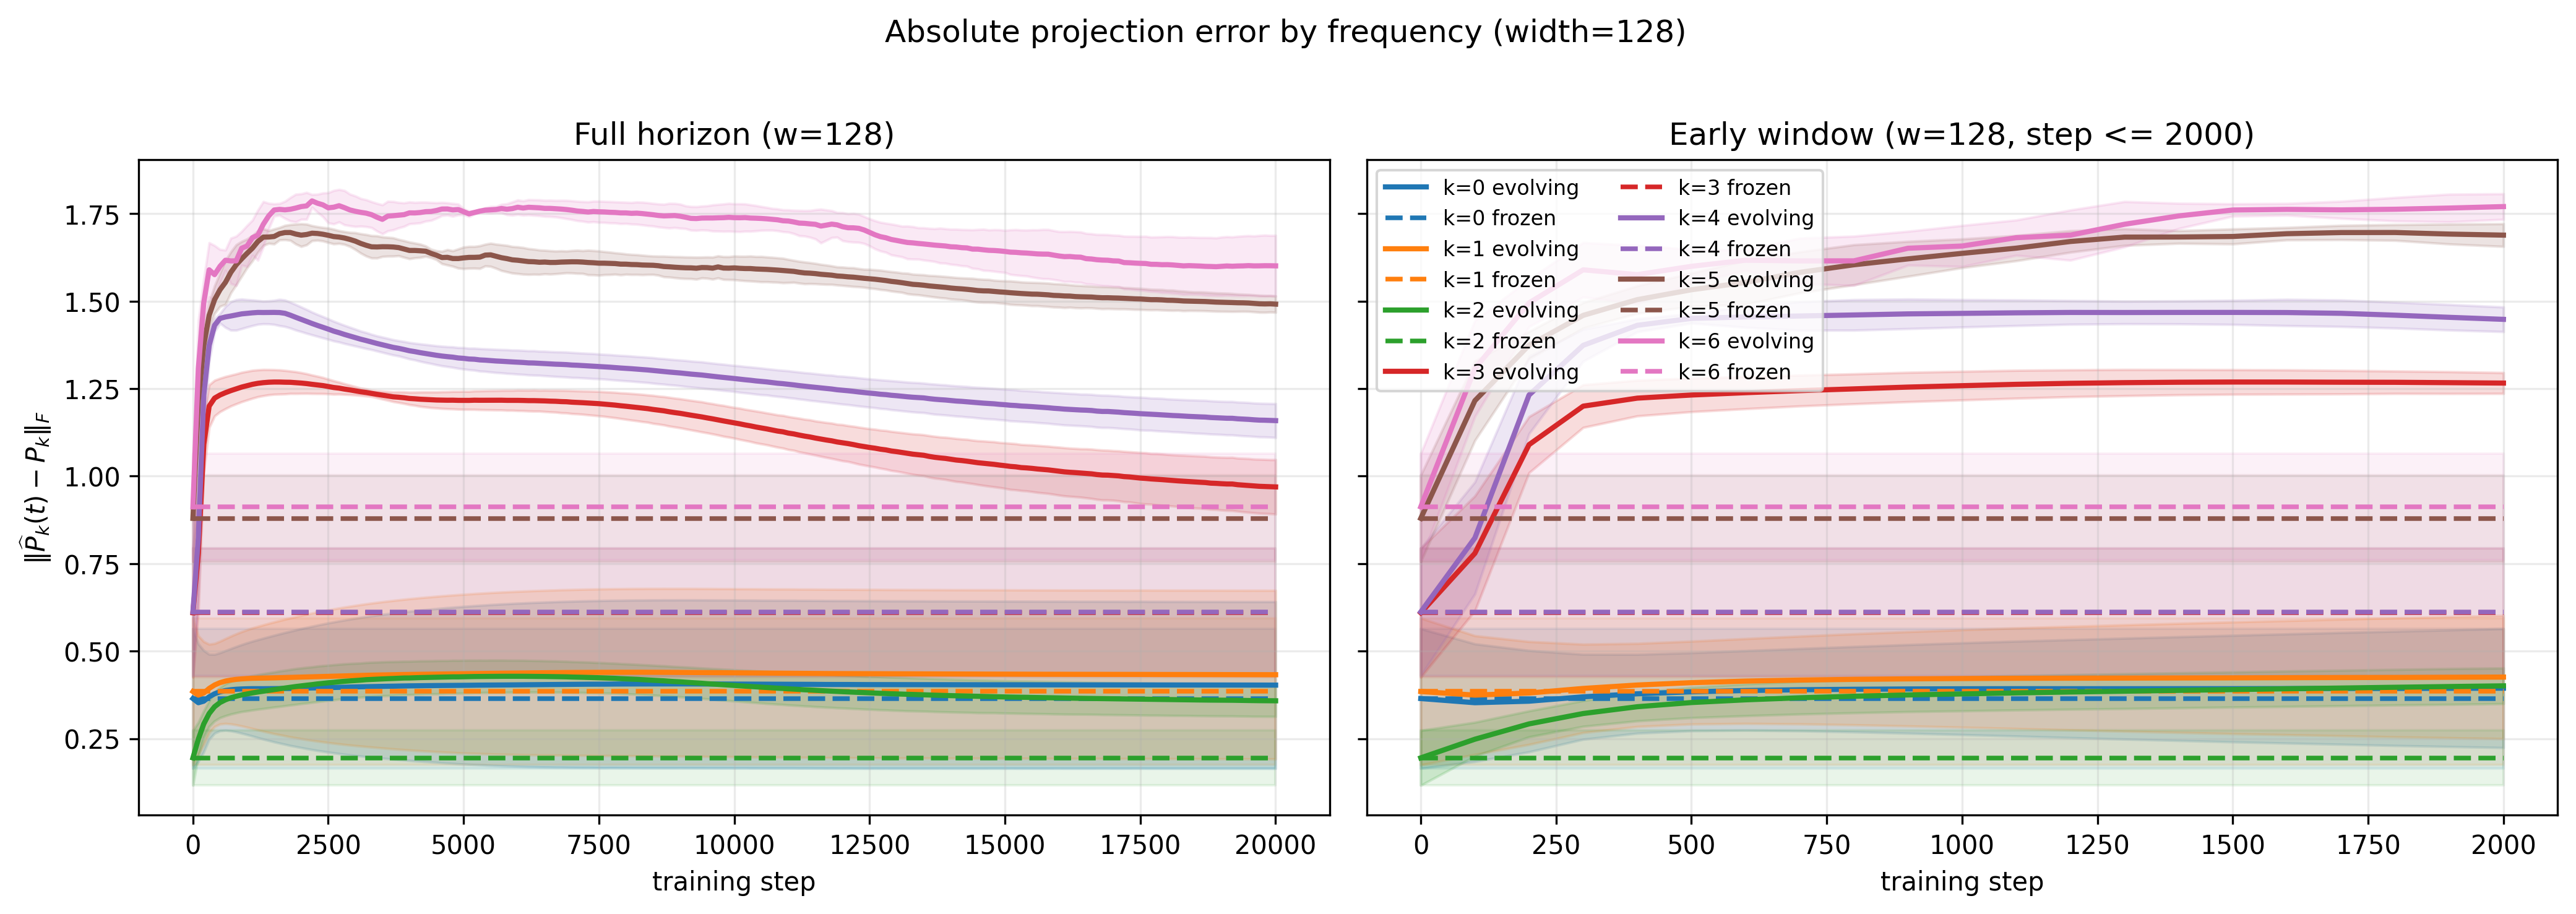
\includegraphics[width=\linewidth]{images/finite_width_evolving_results/projection_error_absolute_by_freq_w128.png}
        \caption{\(w = 128\)}
    \end{subfigure}
    \hfill
    \begin{subfigure}[b]{0.49\linewidth}
        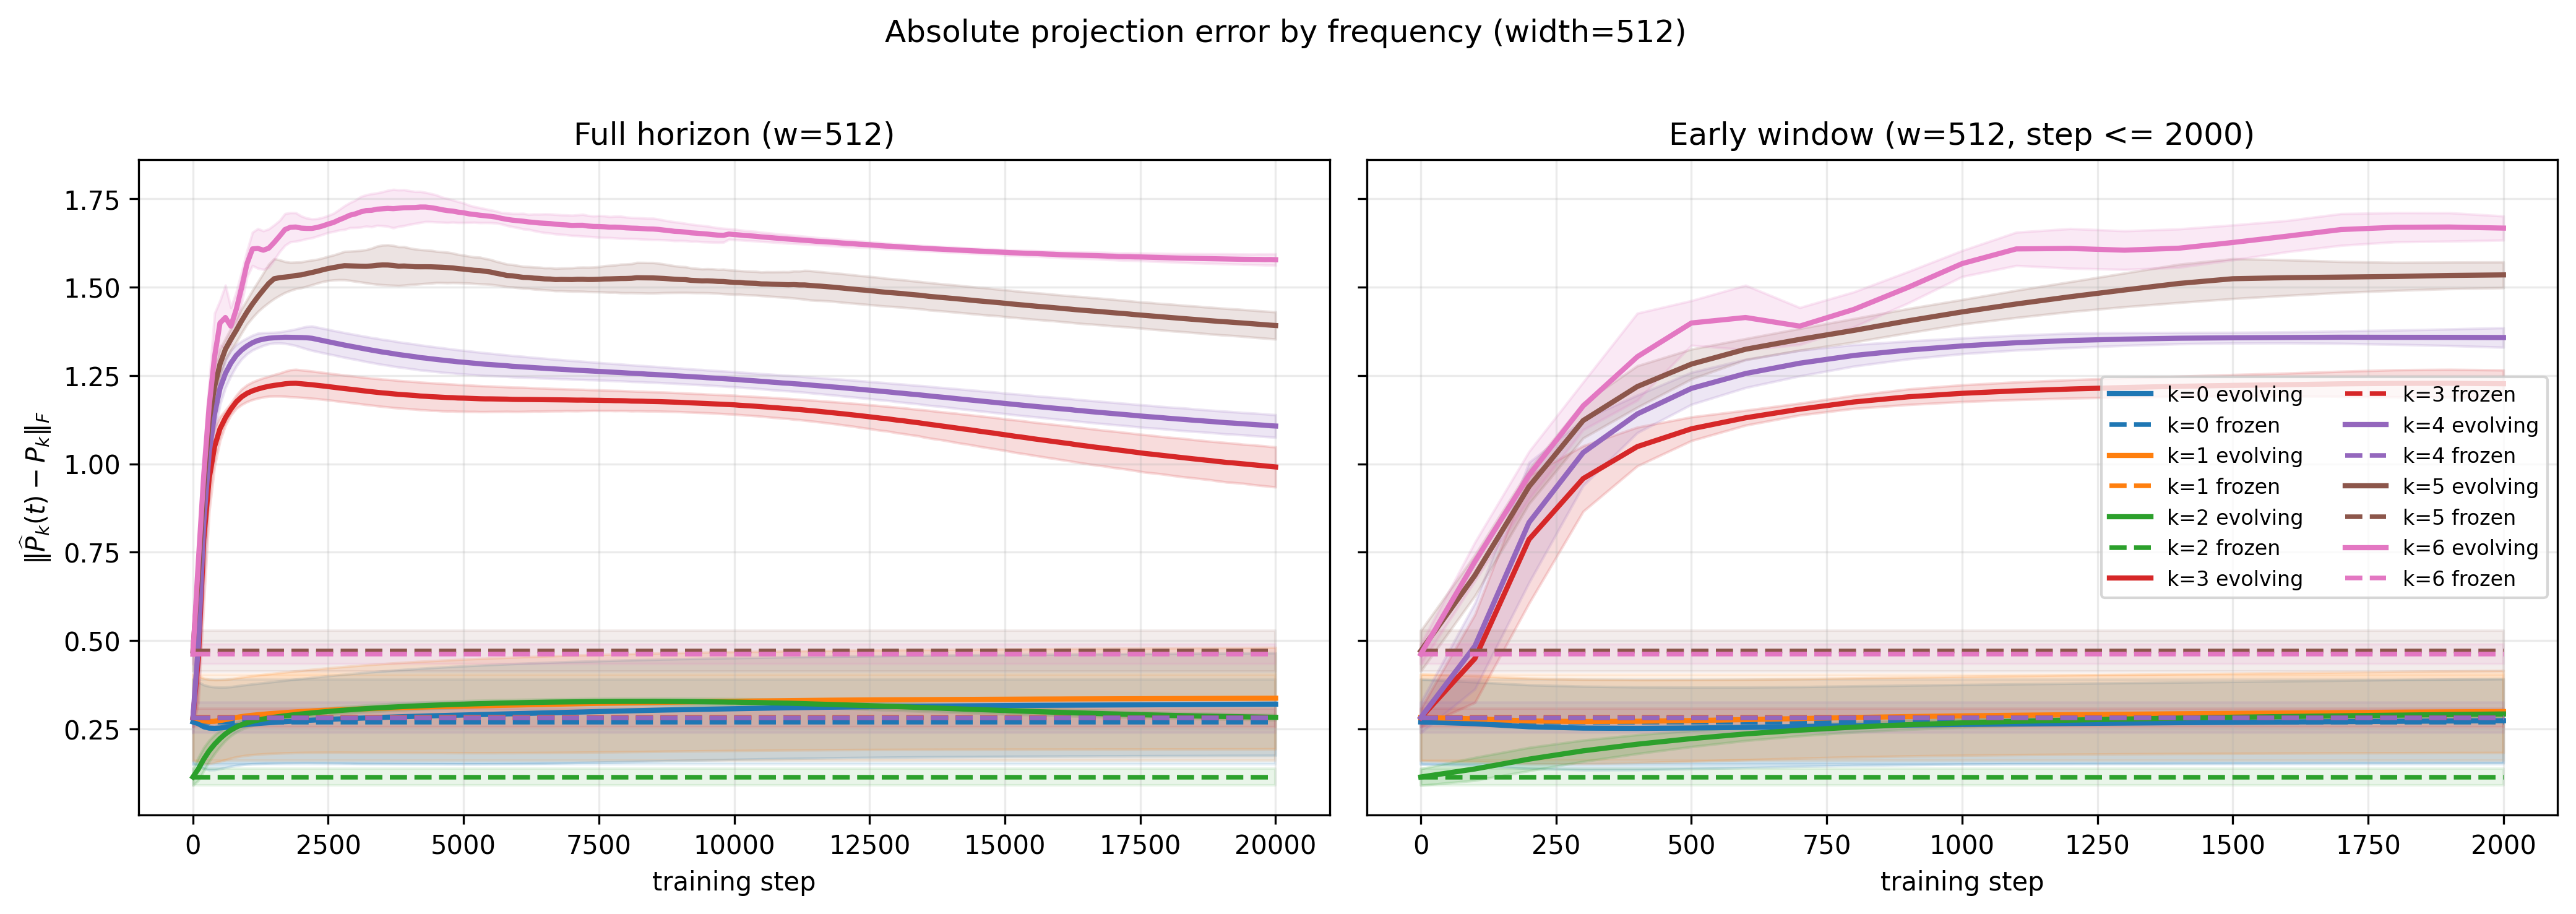
\includegraphics[width=\linewidth]{images/finite_width_evolving_results/projection_error_absolute_by_freq_w512.png}
        \caption{\(w = 512\)}
    \end{subfigure}
    \caption{Absolute projection error \(\|\hat P_k(t)-\hat P_k(0)\|_F\)
        by frequency \(k\), comparing frozen (dashed) and evolving (solid)
        networks at widths 128 and 512.
        Frozen projectors are stable; evolving ones drift, increasingly so at
        low width.}
    \label{fig:app-proj-err}
\end{figure}

% ---------------------------------------------------------------------------
\section{Finite-width evolving: cross-width summary and robustness}
\label{app:add-evolving}

Figure~\ref{fig:app-subspace-grid} shows the full per-subspace story—alignment,
projection error, and spectral strength—across all four widths and six target
frequencies simultaneously.
The pattern is consistent: alignment is high and grows with width; projection
error is moderate and shrinks with width; spectral strength accumulates at
a width-dependent rate.

\begin{figure}[!htbp]
    \centering
    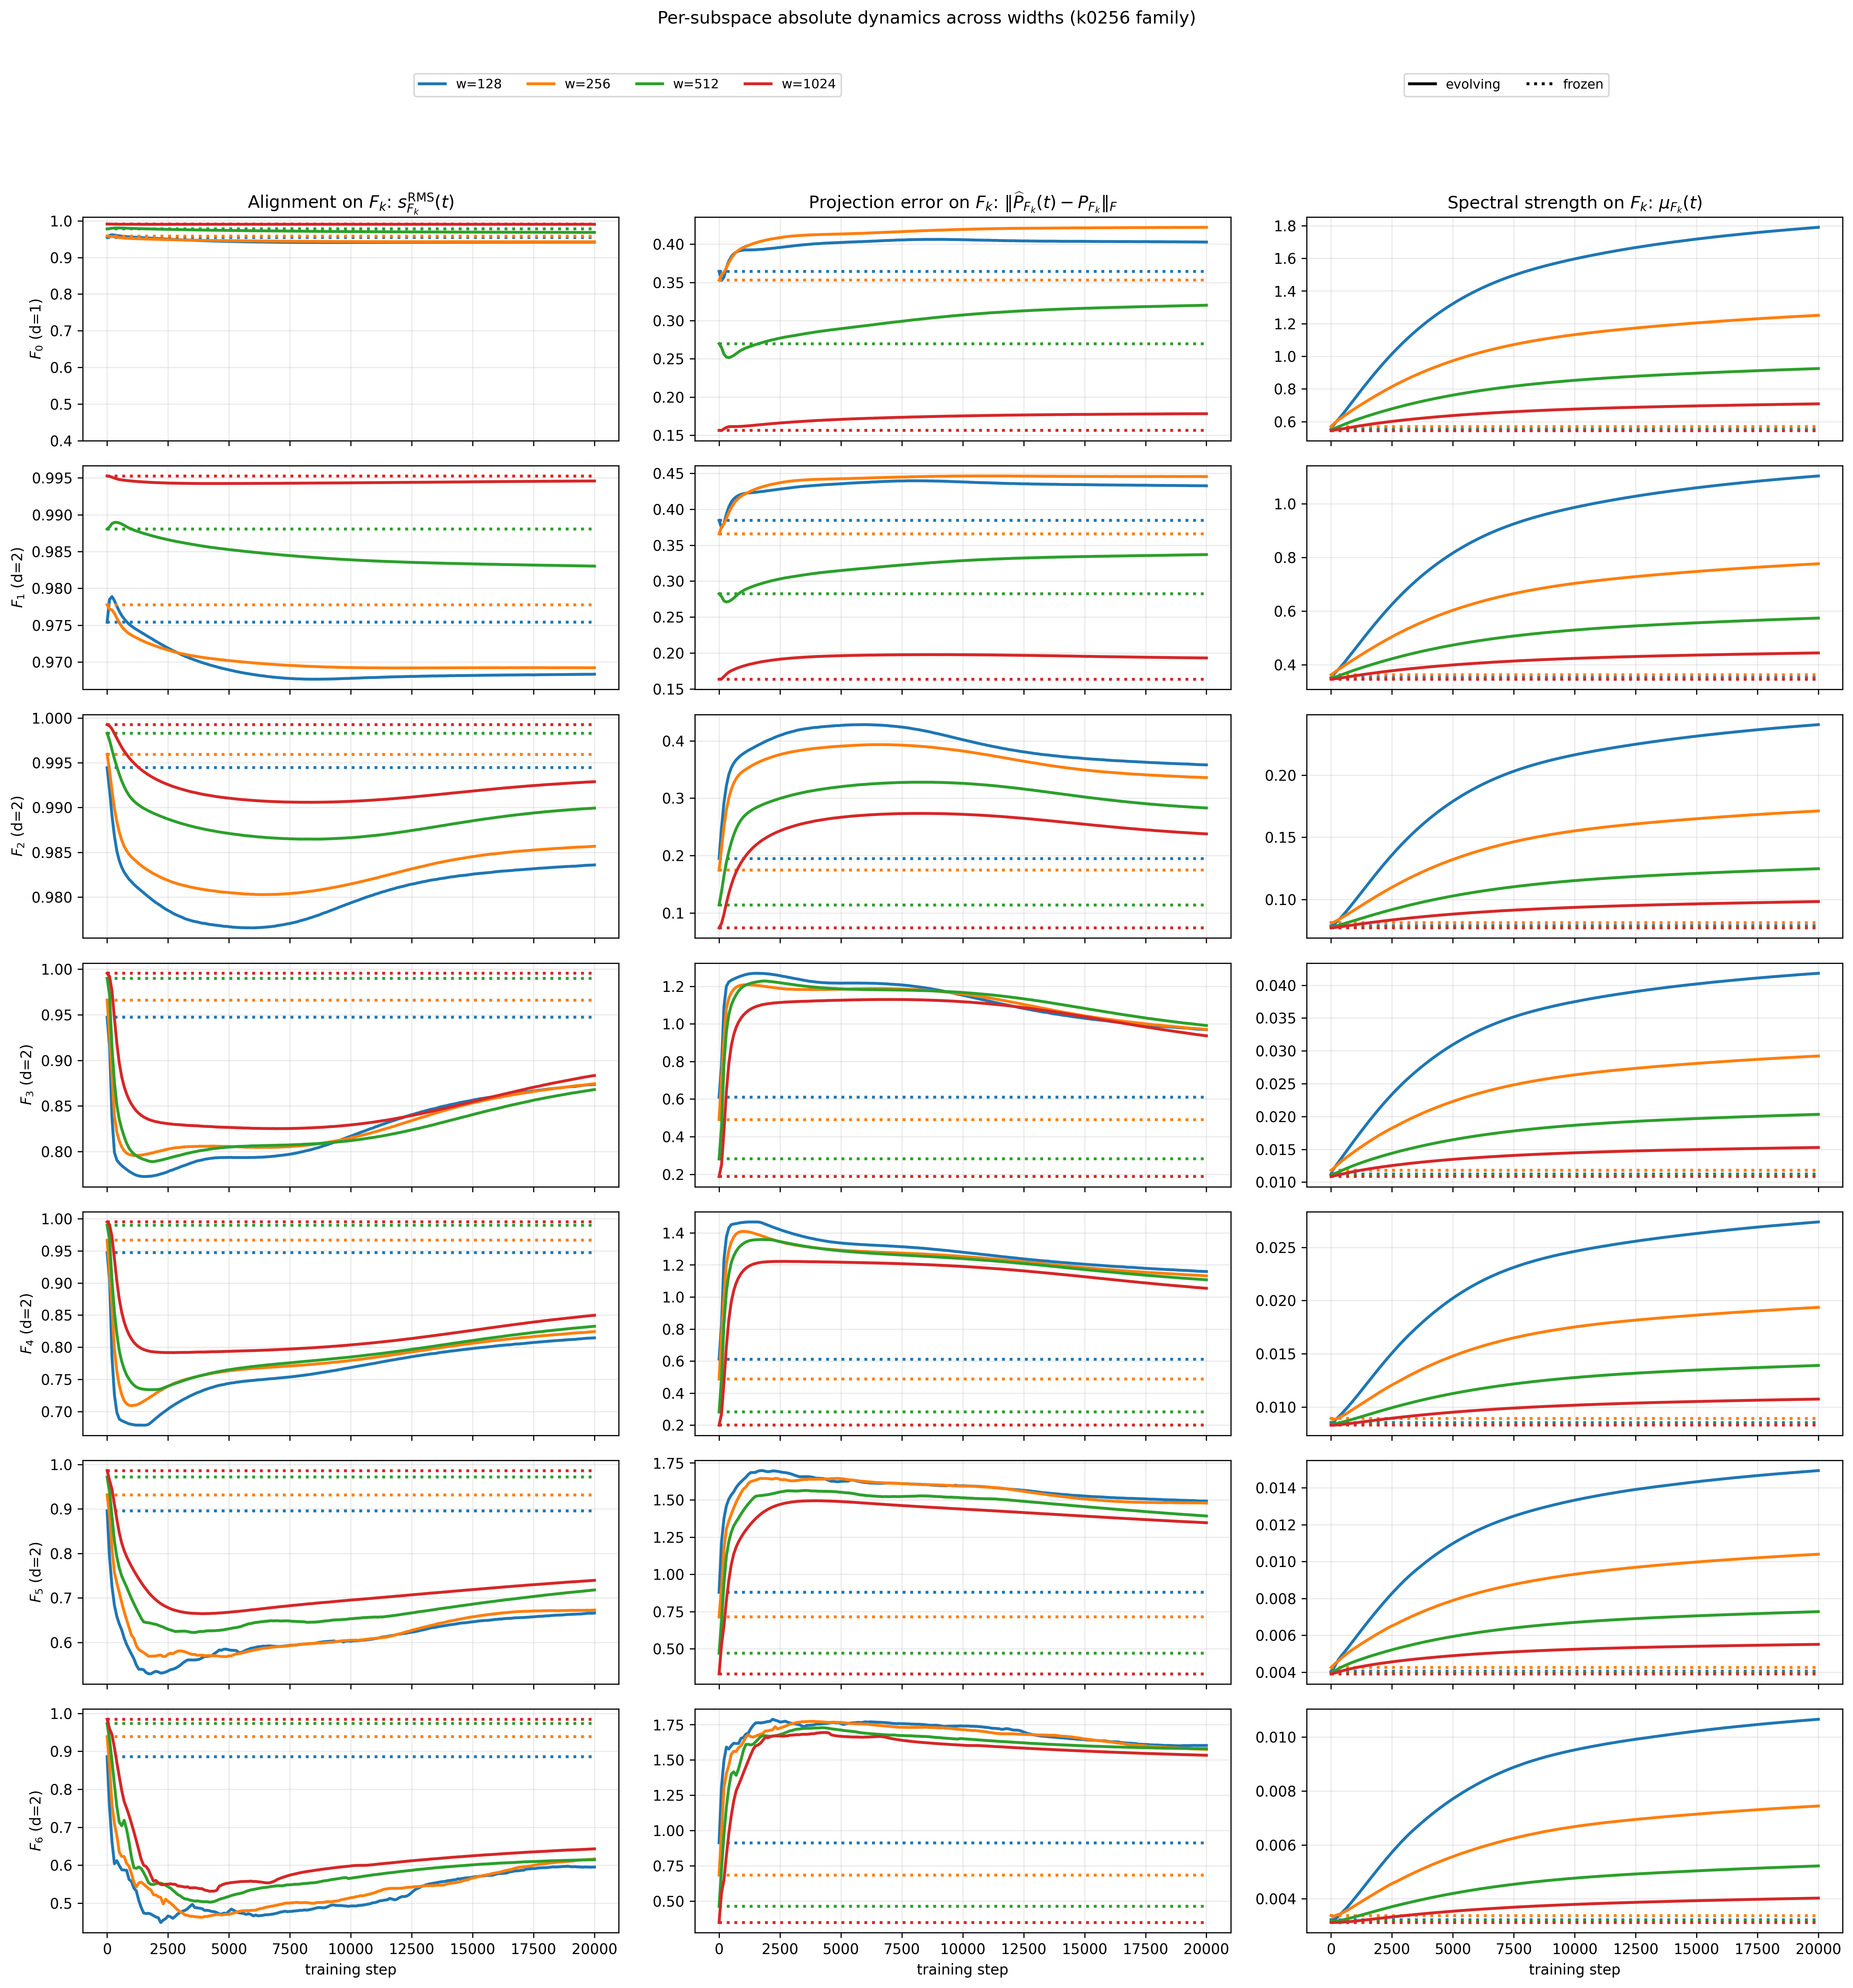
\includegraphics[width=\linewidth]{images/appendix/per_subspace_story_grid_absolute_w128_w256_w512_w1024.png}
    \caption{Per-subspace dynamics across widths \(w \in \{128,256,512,1024\}\)
        (line colours) for each of the six target frequencies (rows).
        Columns show cosine alignment, absolute projection error, and spectral
        strength, for both frozen (dashed) and evolving (solid) networks.}
    \label{fig:app-subspace-grid}
\end{figure}

Figure~\ref{fig:app-equalamp} checks that the spectral ordering of mode decay
is not an artefact of unequal target amplitudes.
When the target is constructed with equal Fourier coefficients across all modes,
the same low-to-high ordering of convergence is observed, confirming that the
effect is driven by the kernel eigenvalue spectrum and not by initialisation.

\begin{figure}[!htbp]
    \centering
    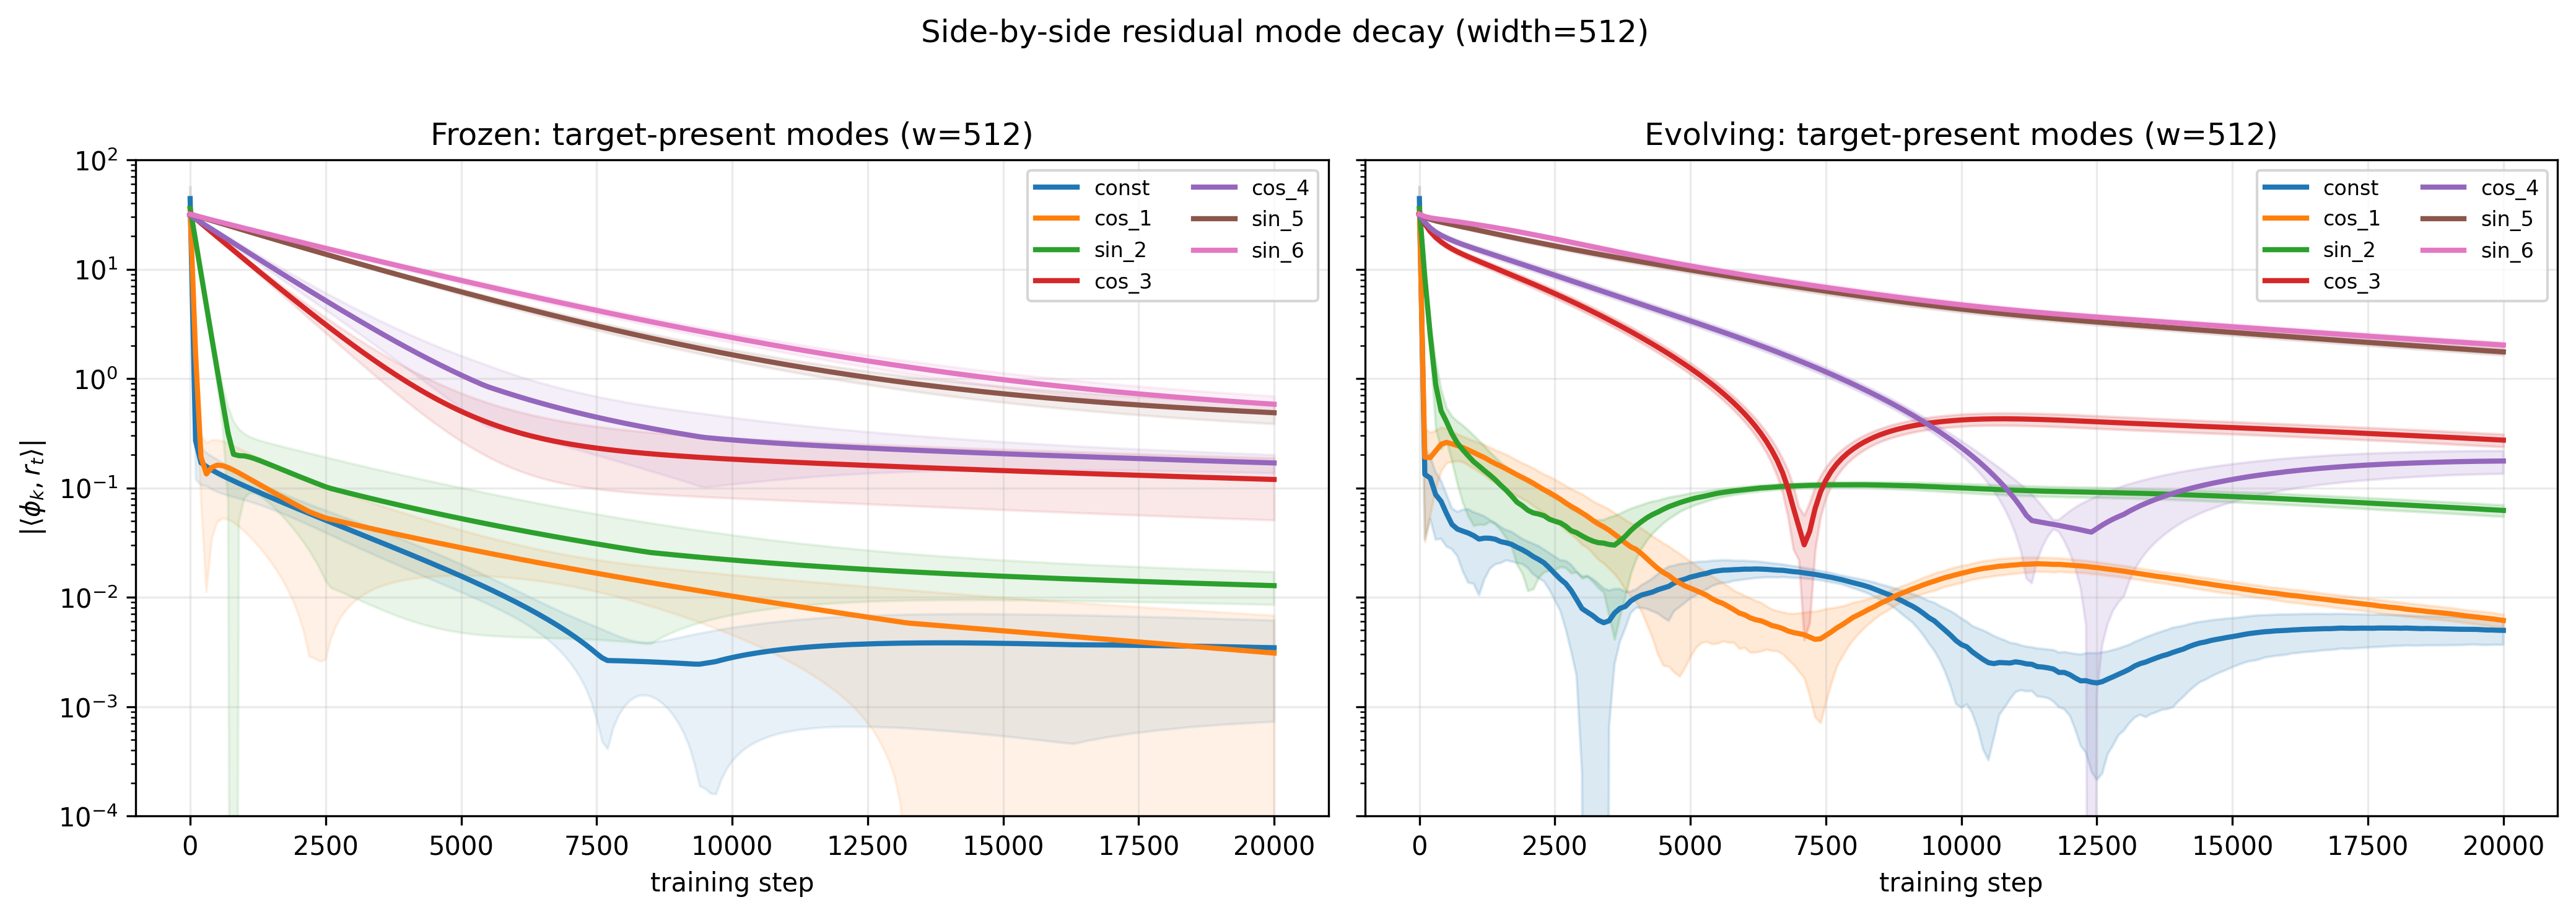
\includegraphics[width=\linewidth]{images/appendix/side_by_side_residual_decay_equalamp_w512.png}
    \caption{Mode residual decay for frozen (left) and evolving (right) networks
        at \(w=512\), using a target with equal Fourier amplitudes across all
        modes.
        The low-frequency modes still converge first, ruling out amplitude bias
        as a confound.}
    \label{fig:app-equalamp}
\end{figure}

Finally, Figure~\ref{fig:app-cumulative} reports the two geometry diagnostics
accumulated over the nested subspaces \(\mathcal F_{\le k}\) rather than per
frequency.
The cumulative RMS-cosine alignment and the cumulative projection error tell the
same story as the per-frequency plots: the evolving kernel (solid) drifts away
from the Fourier reference relative to the frozen baseline (dashed), with the gap
widening as more high-frequency blocks are included.

\begin{figure}[!htbp]
    \centering
    \begin{subfigure}[b]{0.49\linewidth}
        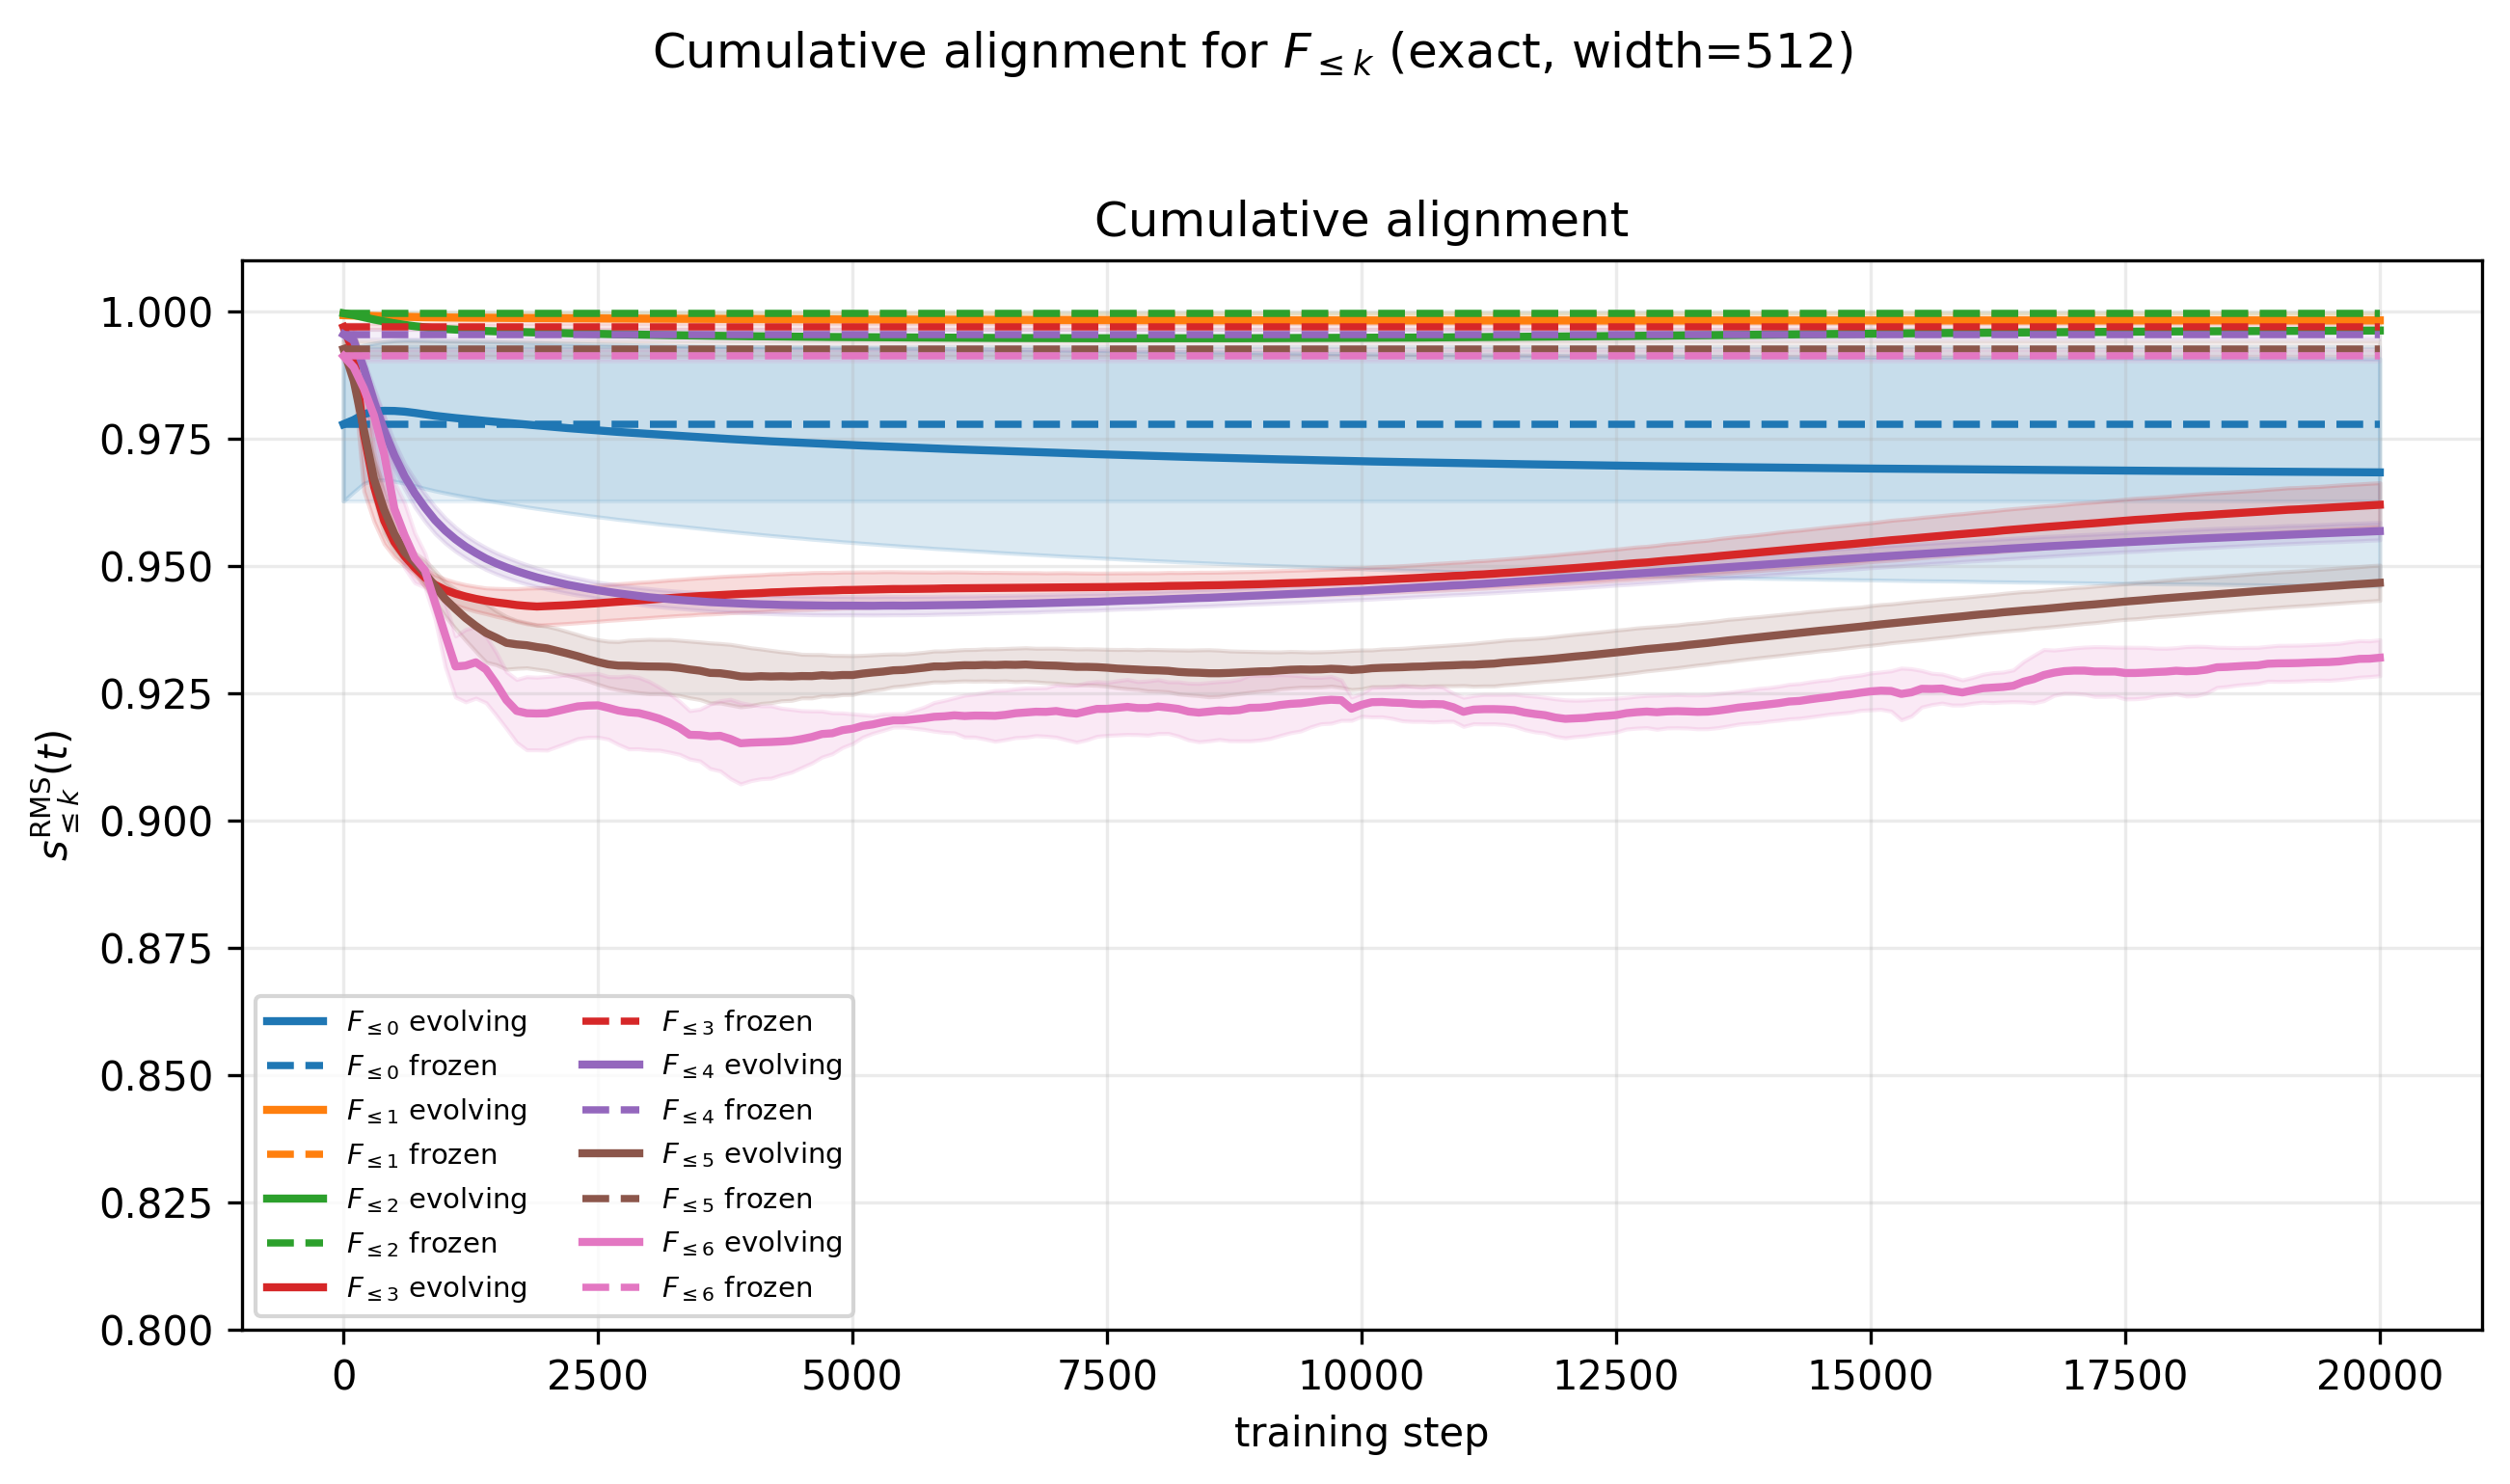
\includegraphics[width=\linewidth]{images/appendix/cumulative_alignment_exact_w512.png}
        \caption{Cumulative RMS-cosine alignment.}
    \end{subfigure}
    \hfill
    \begin{subfigure}[b]{0.49\linewidth}
        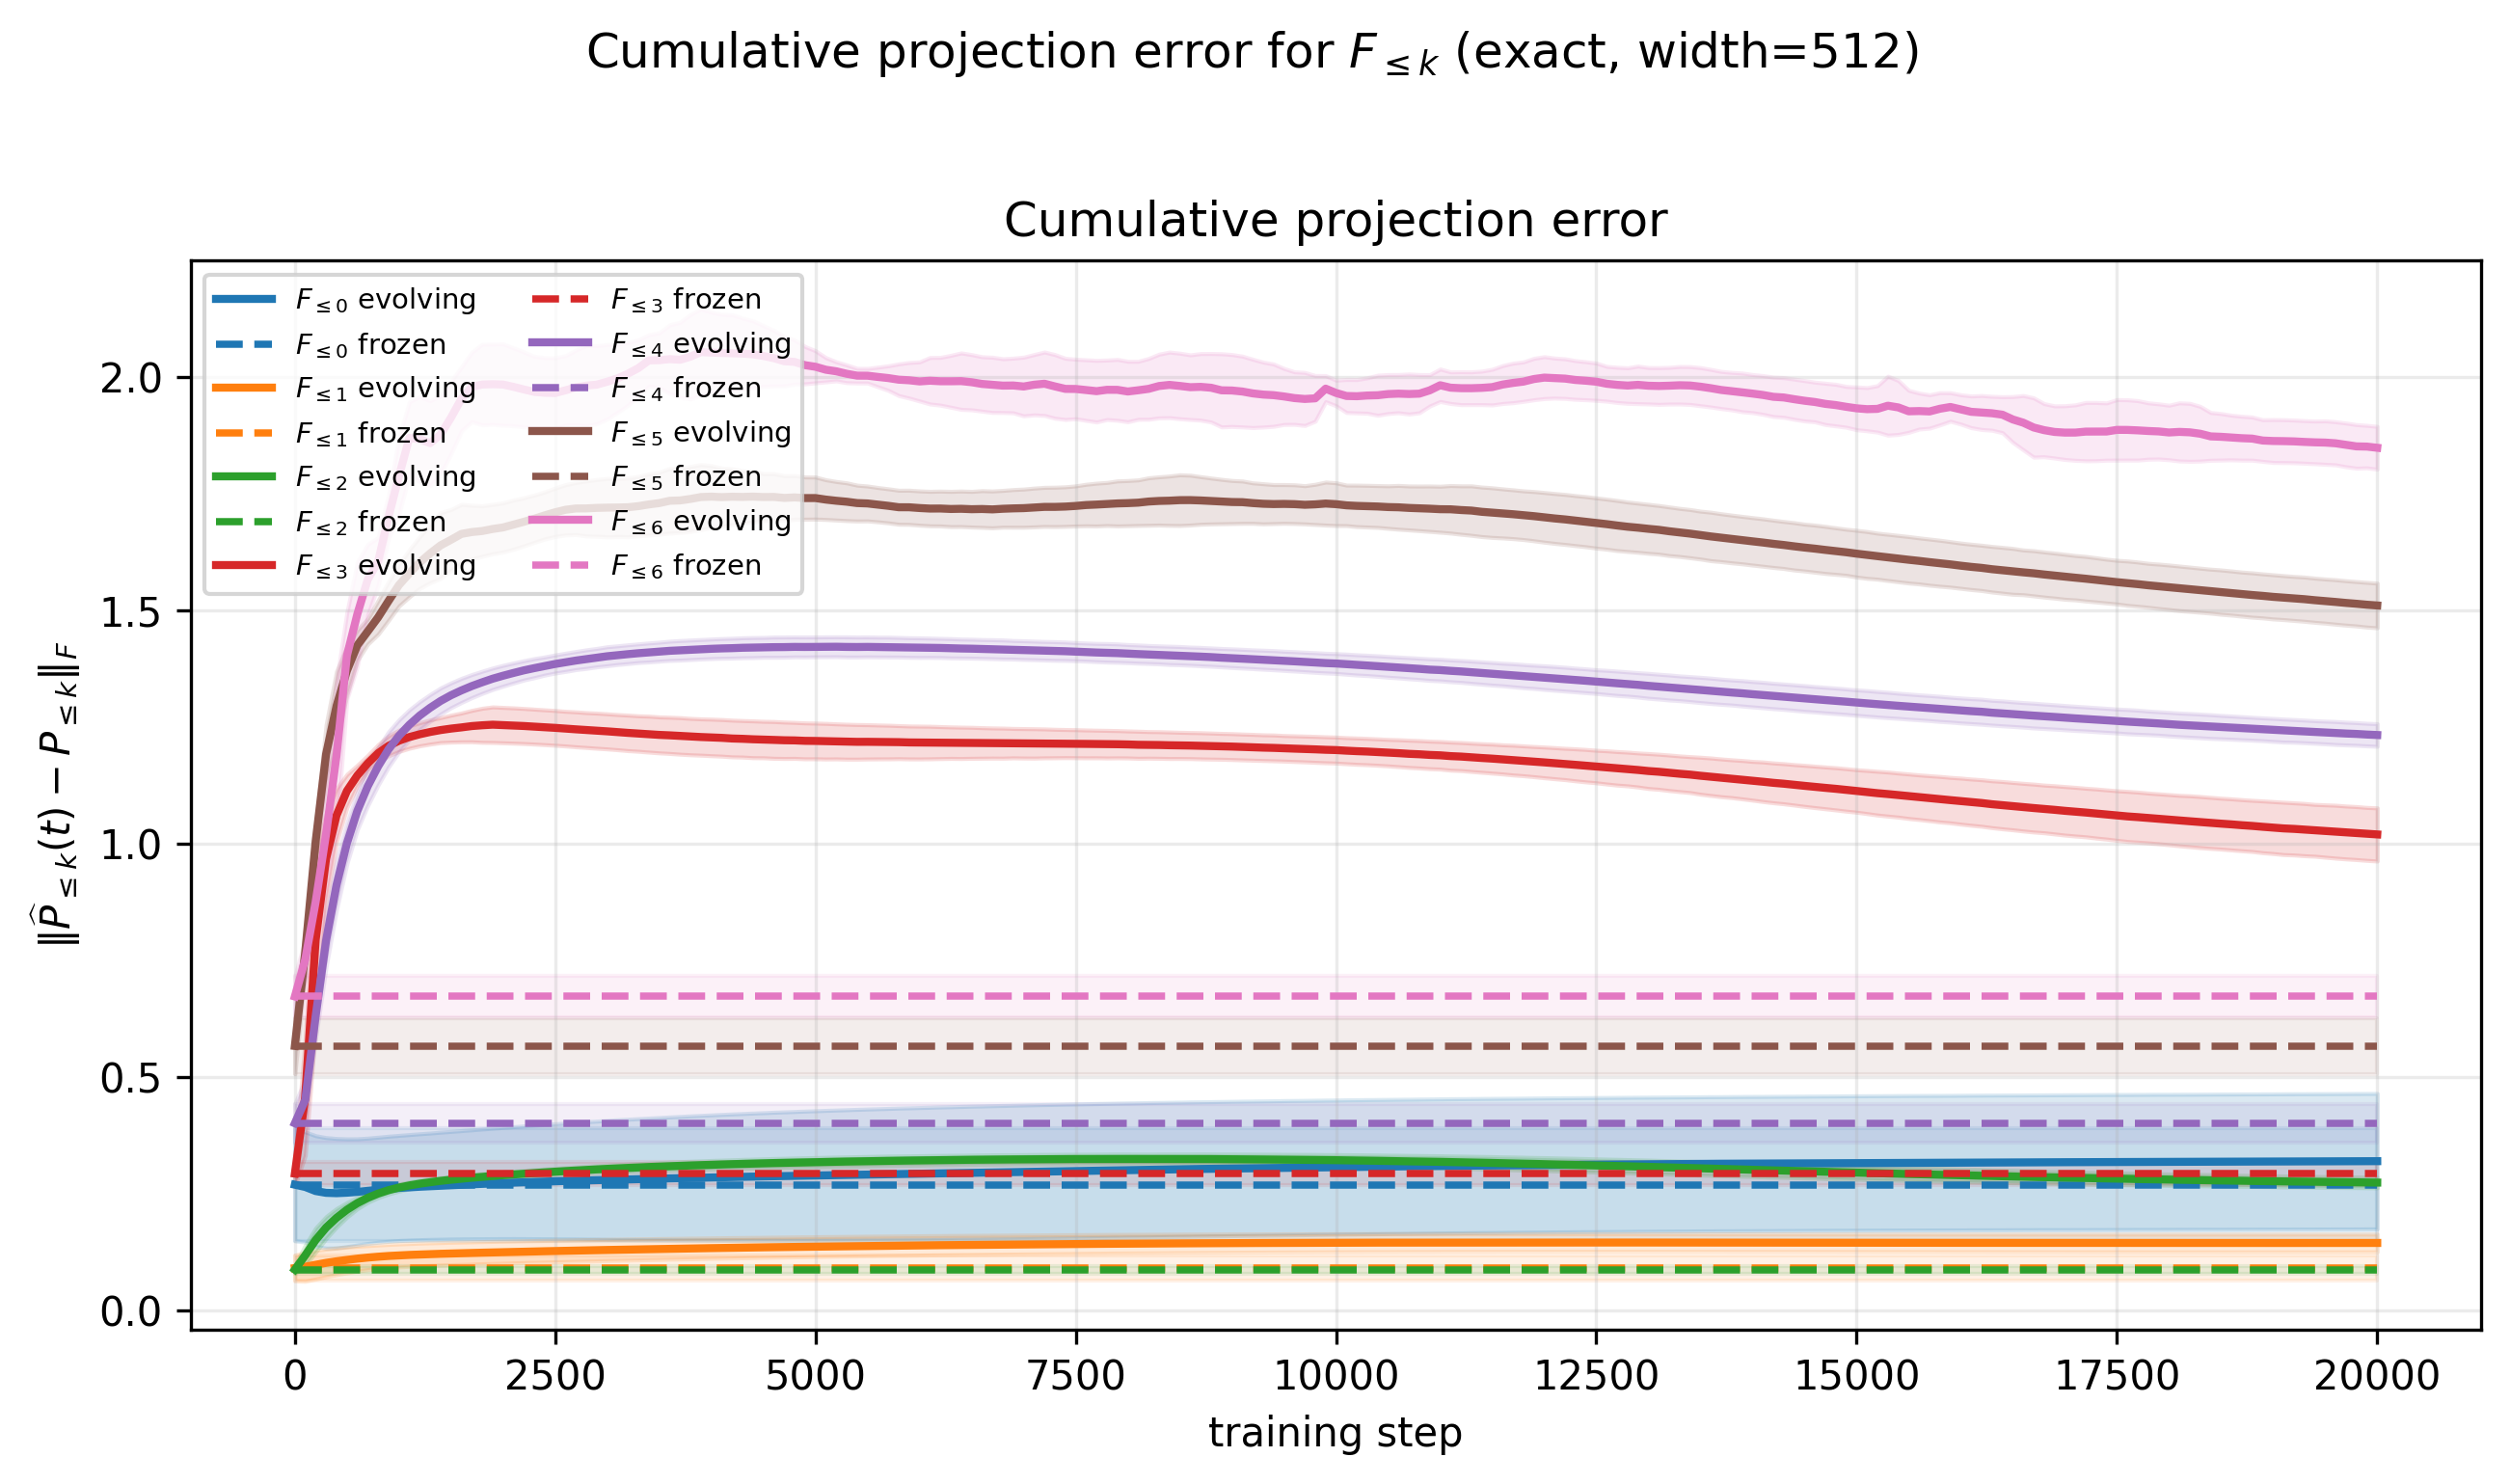
\includegraphics[width=\linewidth]{images/appendix/cumulative_projection_error_exact_w512.png}
        \caption{Cumulative projection error.}
    \end{subfigure}
    \caption{Cumulative geometry diagnostics over the nested subspaces
        \(\mathcal F_{\le k}\) at width \(512\), for frozen (dashed) and evolving
        (solid) networks.
        Left: cumulative RMS-cosine alignment \(S^{\mathrm{RMS}}_{\le k}(t)\).
        Right: cumulative projection error
        \(\|\widehat P_{\le k}(t)-P_{\le k}\|_F\).
        The evolving kernel becomes less Fourier-aligned over training,
        increasingly so as higher-frequency blocks are included.}
    \label{fig:app-cumulative}
\end{figure}

